% Linear and Multilinear Algebra submission manuscript.
% Portable initial-submission layout; compile from this directory with:
%   latexmk -pdf -interaction=nonstopmode -halt-on-error \
%     lma_pseudospectral_connectedness.tex
\documentclass[11pt,a4paper]{article}

\usepackage[T1]{fontenc}
\usepackage{newtxtext}
\usepackage[english]{babel}
\usepackage[margin=1in]{geometry}
\usepackage{mathtools,amsthm}
\usepackage{newtxmath}
\usepackage{booktabs}
\usepackage{graphicx}
\usepackage{microtype}
\usepackage{placeins}
\usepackage[numbers,sort&compress]{natbib}
\usepackage[hidelinks]{hyperref}
\usepackage[capitalise,noabbrev]{cleveref}

\linespread{1.04}
\setlength{\parskip}{0.25em}
\setlength{\parindent}{1.5em}

\allowdisplaybreaks
\graphicspath{{./}}
\DeclareGraphicsExtensions{.pdf,.png,.jpg}
\numberwithin{equation}{section}
\newtheorem{theorem}{Theorem}[section]
\newtheorem{lemma}[theorem]{Lemma}
\newtheorem{proposition}[theorem]{Proposition}

\crefname{appendix}{appendix}{appendices}
\Crefname{appendix}{Appendix}{Appendices}
\crefname{lemma}{lemma}{lemmas}
\Crefname{lemma}{Lemma}{Lemmas}
\crefname{proposition}{proposition}{propositions}
\Crefname{proposition}{Proposition}{Propositions}

\DeclareMathOperator{\diag}{diag}
\DeclareMathOperator{\tridiag}{tridiag}

\newcommand{\C}{\mathbb C}
\newcommand{\R}{\mathbb R}
\newcommand{\ii}{\mathrm i}
\newcommand{\proofstage}[1]{%
  \par\medskip\noindent\textit{#1}\par\nobreak\smallskip}

\newcommand{\Names}{Shanmu Jin}
\newcommand{\Title}{Exact connectedness thresholds and strict order
monotonicity for complex tridiagonal Toeplitz pseudospectra}

\hypersetup{
  pdftitle={\Title},
  pdfauthor={Shanmu Jin},
  pdfsubject={Exact pseudospectral connectedness thresholds, spectral-line
    contraction, and strict matrix-order monotonicity},
  pdfkeywords={pseudospectrum, tridiagonal Toeplitz matrix, nonnormal matrix,
    least singular value, pseudospectral connectedness, matrix-order monotonicity}
}

\begin{document}

\title{\Title}
\author{Shanmu Jin\thanks{Department of Neurosurgery, Peking Union Medical
College Hospital, No.~1 Shuaifuyuan, Dongcheng District, Beijing 100730,
China. Email: \href{mailto:jinshanmu1129@pku.edu.cn}{jinshanmu1129@pku.edu.cn}.
ORCID: \href{https://orcid.org/0009-0009-5346-753X}{0009-0009-5346-753X}.}}
\date{}
\maketitle

\begin{abstract}
We establish three connectedness results for open Euclidean-norm
pseudospectra.  First, for a finite matrix whose spectrum lies on an affine
line, a natural least-singular-value contraction condition forces every
pseudospectral component to be contractible and reduces connectedness to a
one-dimensional barrier.  Second, this principle yields an exact threshold
for the full complex tridiagonal Toeplitz family
\(T_n(\alpha,d,\beta)=\tridiag(\alpha,d,\beta)\).  Set
\(c=\max\{|\alpha|,|\beta|\}\).  When \(c>0\), unitary similarity and affine
transformations reduce the problem to
\(A_n(a)=\tridiag(a,0,1)\), with
\(a=\min\{|\alpha|,|\beta|\}/c\).  In the irreducible nonnormal regime
\(0<a<1\), if \(\gamma_n(a)\) is the real-axis least-singular-value barrier,
then \(\sigma_\varepsilon(T_n)\) is connected exactly when
\(\varepsilon>c\gamma_n(a)\).  Third, the thresholds obey the strict
all-order inequality \(\gamma_{n+1}(a)<\gamma_n(a)\) for every \(n\geq2\).
Thus connectedness persists with increasing order.  Matching bounds of order
\((n+1)a^{n/2}\) give a two-term logarithmic asymptotic for the first
connected order.  The normal boundary has an algebraic threshold, while the
one-sided and scalar cases have zero threshold.
\end{abstract}

\medskip
\noindent\textbf{Keywords:}
pseudospectrum, tridiagonal Toeplitz matrix, nonnormal matrix, least singular
value, pseudospectral connectedness, matrix-order monotonicity.

\smallskip
\noindent\textbf{2020 Mathematics Subject Classification:}
15A18 (primary); 15A60, 15B05, 65F15 (secondary).

\section{Introduction}\label{sec:introduction}

Let \(n\geq1\), \(A\in\C^{n\times n}\), and \(\varepsilon>0\).  The open
Euclidean-norm \(\varepsilon\)-pseudospectrum is
\begin{equation}\label{eq:intro-pseudospectrum}
 \sigma_\varepsilon(A)
 =\sigma(A)\cup
 \{z\in\C\setminus\sigma(A):
   \lVert(zI_n-A)^{-1}\rVert_2>\varepsilon^{-1}\}
 =\{z\in\C:s_{\min}(zI_n-A)<\varepsilon\}.
\end{equation}
Here and throughout, \(I_n\) is the \(n\)-by-\(n\) identity,
\(s_{\min}\) denotes the least singular value, and \(\lVert\cdot\rVert_2\)
is the Euclidean norm on vectors or its induced operator norm on matrices.
Equivalently, \eqref{eq:intro-pseudospectrum} is the union of the spectra of
\(A+\Delta A\) over all complex perturbations satisfying
\(\lVert\Delta A\rVert_2<\varepsilon\)
\cite{TrefethenEmbree2005}.  Pseudospectral components therefore encode
spectral clusters stable under unstructured perturbations.  Their merger is
also related to distance to defectivity: for matrices with distinct
eigenvalues, first-coalescence points are the lowest generalized saddle
points of the least-singular-value function, and their common level equals
the distance to the set of defective matrices in the induced Euclidean
operator norm
\cite{AlamEtAl2011}.  Thus connectedness depends on the global geometry of
the least-singular-value landscape, not on the spectrum alone.

The contribution of this paper is threefold.
\begin{enumerate}
\item \emph{A general spectral-line contraction theorem.}
For a finite matrix with spectrum on an affine line, a natural contraction
condition on least-singular-value sublevel sets makes every pseudospectral
component contractible and reduces connectedness to the largest
one-dimensional barrier between adjacent eigenvalues.

\item \emph{An exact Toeplitz threshold.}
For every \(n\geq2\) and all complex \(\alpha,d,\beta\), we give a
necessary-and-sufficient connectedness criterion for
\(T_n(\alpha,d,\beta)=\tridiag(\alpha,d,\beta)\), including its reducible,
irreducible nonnormal, and normal regimes.

\item \emph{Strict monotonicity at every order.}
In the canonical nonnormal regime \(0<a<1\), the exact thresholds satisfy
\(\gamma_{n+1}(a)<\gamma_n(a)\) for all \(n\geq2\).  Hence connectedness,
once attained, persists at every larger order.
\end{enumerate}

We study the full complex tridiagonal Toeplitz family
\begin{equation}\label{eq:A-matrix}
 T_n(\alpha,d,\beta)=\tridiag(\alpha,d,\beta)
 =\begin{bmatrix}
 d&\beta\\
 \alpha&d&\ddots\\
 &\ddots&\ddots&\beta\\
 &&\alpha&d
 \end{bmatrix},
 \qquad n\geq2,\quad \alpha,d,\beta\in\C,
\end{equation}
where the arguments of \(\tridiag\) are the subdiagonal, diagonal, and
superdiagonal.  Its Euclidean-norm pseudospectral geometry is determined by
the two real quantities
\[
 c=\max\{|\alpha|,|\beta|\},
 \qquad a=\frac{\min\{|\alpha|,|\beta|\}}{c}\in[0,1],
\]
when \(c>0\).  A diagonal unitary, possibly followed by reversal, reduces
\(T_n(\alpha,d,\beta)\) to a translate, rotation, and positive multiple of
the canonical matrix
\begin{equation}\label{eq:canonical-matrix}
 A_n(a)=\tridiag(a,0,1).
\end{equation}
The parameter in \eqref{eq:canonical-matrix} separates three regimes:
\(a=0\) is the one-sided nilpotent-shift boundary, \(0<a<1\) is the
irreducible nonnormal regime, and \(a=1\) is the normal boundary.  The scalar
case \(c=0\) is treated separately.

For \(0<a<1\), write
\begin{equation}\label{eq:intro-gamma}
 \gamma_n(a)=\max_{|x|\leq2\sqrt a\cos(\pi/(n+1))}
 s_{\min}(xI_n-A_n(a)).
\end{equation}
Then \(\sigma_\varepsilon(T_n(\alpha,d,\beta))\) is connected if and only if
\(\varepsilon>c\gamma_n(a)\).

The proof compares global barriers on spectral intervals that vary with the
matrix order.  Diagonal similarity identifies the spectrum but has Euclidean
condition number \(a^{-(n-1)/2}\); interlacing is pointwise, while the barrier
maximizes over moving gaps whose central geometry changes with parity.
Toeplitz asymptotics describe the eventual scale, whereas adjacent-order
monotonicity requires a finite-order comparison.

The Toeplitz background begins with the Schmidt--Spitzer characterization of
the eigenvalue limit set for matrices generated by a Laurent polynomial
\cite{SchmidtSpitzer1960}.  Reichel and Trefethen analyze finite
non-Hermitian Toeplitz eigenvalues, resolvent norms, and pseudospectra
\cite{ReichelTrefethen1992}.  For large truncated Wiener--Hopf operators,
B\"ottcher establishes limiting results for inverse norms, pseudospectra, and
singular values \cite{Bottcher1994}; a book-length treatment of banded
Toeplitz spectral theory, including resolvents, pseudospectra, singular
values, and structured perturbations, is given in
\cite{BottcherGrudsky2005}.  Closed-form spectral, sensitivity, and
pseudospectral properties of tridiagonal Toeplitz matrices are developed in
\cite{NoschesePasquiniReichel2013}, while algorithms for Toeplitz-structured
pseudospectra and their extreme points are studied in
\cite{ButtaGuglielmiNoschese2012}.

Recent directions include convergent spectral and pseudospectral inclusion
sets for banded and band-dominated operators \cite{ChandlerWildeEtAl2024}
and individual asymptotic expansions for all eigenvalues in a non-Hermitian
tetradiagonal Toeplitz class \cite{BogoyaGascaGrudsky2025}.  Spectra and
pseudospectra of tridiagonal \(k\)-Toeplitz operators and matrices are studied
in \cite{AmmariEtAl2025}; the corrected finite-matrix pseudospectral limit is
given in \cite{AmmariCorrigendum2026}.

At the level of topology, pseudospectral optimization and component geometry
are developed in \cite{BurkeLewisOverton2003}.  Pseudospectral growth is
related to spectral conditioning, and the first loss of \(n\) components is
shown to equal the distance to matrices with multiple eigenvalues in
\cite{BurkeLewisOverton2007}.  Alam, Bora, Byers, and Overton further identify
first-coalescence points as lowest generalized saddle points and relate their
level to distance to defectivity \cite{AlamEtAl2011}.

A parallel line of work quantifies eigenvalue instability in random
non-self-adjoint matrices \cite{Davies2001}, analyzes pseudospectra,
exponential resolvent growth, and localization in random bidiagonal models
\cite{TrefethenContediniEmbree2001}, and exhibits recent Toeplitz-like
examples of spectral instability \cite{Bottcher2024}.  In non-Hermitian
lattice problems, Ammari et al. prove exponential edge localization for the
nontrivial eigenvectors of a finite gauge-capacitance chain
\cite{AmmariEtAl2024}; Kiorpelidis and Makris
identify a critical order beyond which the initially separate
pseudospectral clouds form a single cloud \cite{KiorpelidisMakris2025}; and
Sirker uses pseudospectra to separate nonnormal spectral instability and the
skin effect from stable topological information \cite{Sirker2026}.

Together these works provide limiting sets, computable enclosures, structured
perturbation models, eigenvalue asymptotics, and general coalescence
principles.  The present result complements them with an exact finite-order
connectedness criterion for the full complex tridiagonal Toeplitz family and
a strict adjacent-order comparison of its Euclidean-norm barriers, organized
by the spectral-line contraction theorem.

For \(0<a<1\), the threshold satisfies
\begin{equation}\label{eq:intro-barrier-order}
 \gamma_n(a)\asymp_a(n+1)a^{n/2},
\end{equation}
with an optimal factor \(n+1\); these bounds yield a two-term logarithmic
asymptotic for the first connected order.  At \(a=1\), the barrier is half
the largest adjacent eigenvalue gap and has order \((n+1)^{-1}\); at \(a=0\),
it vanishes.  Scalar matrices also have zero threshold.  Thus the nonnormal
interior, normal boundary, and zero-threshold cases have
exponential--polynomial, algebraic, and zero scales, respectively.

\Cref{sec:topological-reduction} proves this topological principle, and
\cref{sec:main-results} performs the unitary--affine reduction and states the
classification.  The Toeplitz-specific proof occupies
\crefrange{sec:vertical}{sec:topology-bounds}: vertical monotonicity gives the
real-axis criterion, signed-pencil and chord arguments prove strict
matrix-order comparison, and rectangular factorizations give the two-sided
bounds.  The algebraic certificates are collected in
\crefrange{app:vertical-certificate}{app:central-certification}; numerical
illustrations and broader implications appear in
\cref{sec:numerics,sec:discussion}.

\section{A vertical-monotonicity principle}
\label{sec:topological-reduction}

This section isolates the topology from the Toeplitz calculation.  Let
\(n\geq1\), let \(B\in\C^{n\times n}\) have real spectrum, and put
\[
 h_B(x,y)=s_{\min}((x+\ii y)I_n-B),\qquad x,y\in\R.
\]
We say that \(B\) has the \emph{vertical contraction property} if
\begin{equation}\label{eq:abstract-vertical-property}
 h_B(x,ty)\leq h_B(x,y)
 \qquad(x,y\in\R,\ 0\leq t\leq1).
\end{equation}
For a real matrix, \eqref{eq:abstract-vertical-property} holds whenever
\(y\mapsto h_B(x,y)\) is nondecreasing on \([0,\infty)\), since singular
values are invariant under complex conjugation.

Write
\[
 \lambda_-(B)=\min\sigma(B),\qquad
 \lambda_+(B)=\max\sigma(B),
\]
and define the real-axis barrier
\begin{equation}\label{eq:abstract-barrier}
 \Gamma(B)=\max_{\lambda_-(B)\leq x\leq\lambda_+(B)}
 s_{\min}(xI_n-B).
\end{equation}
The maximum exists by continuity and equals the largest pointwise backward
error: for each \(x\),
\begin{equation}\label{eq:backward-error-abstract}
 s_{\min}(xI_n-B)=
 \min\{\lVert\Delta B\rVert_2:x\in\sigma(B+\Delta B)\}.
\end{equation}
Identity \eqref{eq:backward-error-abstract} follows because, if
\((xI_n-B-\Delta B)v=0\) for a unit vector \(v\), then
\(s_{\min}(xI_n-B)\leq\lVert\Delta B\rVert_2\).  Conversely, unit singular
vectors satisfying \((xI_n-B)v=s_{\min}(xI_n-B)u\) yield the minimizing
rank-one perturbation \(\Delta B=s_{\min}(xI_n-B)uv^*\).

We use the following standard component fact in a form that applies to every
finite matrix \cite{BurkeLewisOverton2003,TrefethenEmbree2005}.

\begin{lemma}[Eigenvalue in every component]\label[lemma]{lem:component}
Let \(n\geq1\), \(M\in\C^{n\times n}\), and \(\varepsilon>0\).  Every connected
component of \(\sigma_\varepsilon(M)\) contains an eigenvalue of \(M\).
\end{lemma}

\begin{proof}
The estimate
\(s_{\min}(zI_n-M)\geq |z|-\lVert M\rVert_2\) makes the pseudospectrum
bounded.  Let \(\mathcal C\) be a component containing no eigenvalue.  If an
eigenvalue belonged to \(\overline{\mathcal C}\), continuity of the least
singular value would give a pseudospectral ball meeting \(\mathcal C\), and
maximality would put that eigenvalue in \(\mathcal C\).  Thus
\(\overline{\mathcal C}\) lies in the resolvent set.  On a neighborhood of
this compact set, \(z\mapsto\lVert(zI_n-M)^{-1}\rVert_2\) is continuous and
subharmonic.  It is at most \(\varepsilon^{-1}\) on
\(\partial\mathcal C\), whereas it is greater than
\(\varepsilon^{-1}\) in \(\mathcal C\).  The maximum principle gives a
contradiction.
\end{proof}

\begin{theorem}[Vertical topology theorem]\label{thm:vertical-topology}
Let \(n\geq1\).  If \(B\in\C^{n\times n}\) has real spectrum and satisfies
\eqref{eq:abstract-vertical-property}, then, for every
\(\varepsilon>0\), each connected component of
\(\sigma_\varepsilon(B)\) is contractible, and
\begin{equation}\label{eq:abstract-connectedness}
 \sigma_\varepsilon(B)\text{ is connected}
 \quad\Longleftrightarrow\quad
 [\lambda_-(B),\lambda_+(B)]\subset\sigma_\varepsilon(B)
 \quad\Longleftrightarrow\quad
 \varepsilon>\Gamma(B).
\end{equation}
If \(\Gamma(B)>0\), then at the positive level
\(\varepsilon=\Gamma(B)\), a maximizing real point is excluded from the
open pseudospectrum.
\end{theorem}

\begin{proof}
Put \(\Omega=\sigma_\varepsilon(B)\).  By
\eqref{eq:abstract-vertical-property},
\[
 \mathcal H_t(x+\ii y)=x+\ii(1-t)y,
 \qquad 0\leq t\leq1,
\]
maps \(\Omega\) into itself.  For any component \(\mathcal C\), the path
\(t\mapsto\mathcal H_t(z)\) cannot leave \(\mathcal C\).  Since
\(\mathcal H_t\) fixes the real axis,
\(\mathcal H_1(\mathcal C)=\mathcal C\cap\R\), and
\(\mathcal H_t|_{\mathcal C}\) is a strong deformation retraction onto this
intersection.  It is nonempty by
\cref{lem:component}; it is connected as the continuous image
\(\mathcal H_1(\mathcal C)\), and is therefore an interval.  Thus
\(\mathcal C\) is contractible.

If \(\Omega\) is connected, then \(\Omega\cap\R\) is an interval containing
all eigenvalues and hence their convex hull.  Conversely, if that convex
hull lies in \(\Omega\), it belongs to one component and contains every
eigenvalue.  By \cref{lem:component}, no other component can exist.  This
proves the first equivalence in \eqref{eq:abstract-connectedness}; the second
is exactly the strict sublevel definition and \eqref{eq:abstract-barrier}.
\end{proof}

Translation, rotation, and positive scaling translate, rotate, and scale the
pseudospectrum and its barrier.  The theorem therefore extends from the real
axis to any affine spectral line and applies to every matrix in
\eqref{eq:A-matrix}.

\section{Complex tridiagonal Toeplitz matrices and main results}
\label{sec:main-results}

We first normalize the phases, orientation, diagonal, and overall scale in
\eqref{eq:A-matrix}.  Let
\(V_n=\tridiag(0,0,1)\), let \(J_n\) be the reversal permutation matrix,
and, for \(|q|=1\), put
\[
 \mathsf D_n(q)=\diag(1,q,\ldots,q^{n-1}).
\]

\begin{proposition}[Unitary--affine reduction]\label[proposition]{prop:complex-reduction}
Let \(n\geq2\), \(c=\max\{|\alpha|,|\beta|\}>0\), and
\(a=\min\{|\alpha|,|\beta|\}/c\).  There are a unitary matrix \(S_n\) and
a unimodular number \(\omega\) such that
\begin{equation}\label{eq:complex-unitary-reduction}
 S_n^*T_n(\alpha,d,\beta)S_n=dI_n+c\omega A_n(a).
\end{equation}
Consequently, for every \(\varepsilon>0\),
\begin{equation}\label{eq:complex-pseudospectrum-reduction}
 \sigma_\varepsilon(T_n(\alpha,d,\beta))
 =d+c\omega\,\sigma_{\varepsilon/c}(A_n(a)).
\end{equation}
\end{proposition}

\begin{proof}
First suppose \(0<|\alpha|\leq|\beta|\).  Write
\(u_\alpha=\alpha/|\alpha|\) and \(u_\beta=\beta/|\beta|\).  Choose
\(|q|=1\) with \(q^2=u_\alpha\overline{u_\beta}\), and put
\(\omega=u_\beta q=u_\alpha q^{-1}\).  Direct multiplication gives
\[
 \mathsf D_n(q)^*T_n(\alpha,d,\beta)\mathsf D_n(q)
 =dI_n+|\beta|\omega A_n(|\alpha|/|\beta|).
\]
If \(|\alpha|>|\beta|>0\), first conjugate by \(J_n\), which interchanges
the two off-diagonals, and apply the preceding case.  If \(\alpha=0\) and
\(\beta\ne0\), take \(S_n=I_n\) and \(\omega=\beta/|\beta|\); if
\(\beta=0\) and \(\alpha\ne0\), take \(S_n=J_n\) and
\(\omega=\alpha/|\alpha|\).  Applying the singular-value transformation in
\eqref{eq:complex-unitary-reduction} gives
\eqref{eq:complex-pseudospectrum-reduction}, because unitary conjugation
preserves singular values, while
\[
 \sigma_\varepsilon(dI_n+c\omega A)
 =d+c\omega\,\sigma_{\varepsilon/c}(A).
\]
\end{proof}

The boundary thresholds follow directly.  Define
\begin{equation}\label{eq:normal-threshold}
 \eta_n=
 \begin{cases}
  2\sin\dfrac{\pi}{2(n+1)},&n\text{ even},\\[6pt]
  \sin\dfrac{\pi}{n+1},&n\text{ odd}.
 \end{cases}
\end{equation}

\begin{proposition}[Reducible and normal boundaries]
\label[proposition]{prop:boundary-cases}
Let \(n\geq2\) and \(\varepsilon>0\).
\begin{enumerate}
\item If \(\alpha=\beta=0\), then
\(\sigma_\varepsilon(T_n)=\{z:|z-d|<\varepsilon\}\).
If exactly one off-diagonal is nonzero, then
\(\sigma_\varepsilon(T_n)\) is also an open disk centered at \(d\).
In both cases it is connected and contractible for every \(n\); its
connectedness threshold is zero.
\item If \(|\alpha|=|\beta|=c>0\), then every pseudospectral component is
contractible and
\begin{equation}\label{eq:normal-connectedness}
 \sigma_\varepsilon(T_n)\text{ is connected}
 \quad\Longleftrightarrow\quad \varepsilon>c\eta_n.
\end{equation}
Moreover, \(\eta_{n+1}<\eta_n\) for every \(n\geq2\), and
\begin{equation}\label{eq:normal-error-bound}
 0\leq \frac{\pi}{n+1}-\eta_n
 \leq \frac{\pi^3}{6(n+1)^3}.
\end{equation}
In particular,
\begin{equation}\label{eq:normal-asymptotic}
 \eta_n=\frac{\pi}{n+1}+O(n^{-3}).
\end{equation}
\end{enumerate}
\end{proposition}

\begin{proof}
The scalar case follows directly.  If exactly one off-diagonal is nonzero,
\cref{prop:complex-reduction} reduces the matrix to the nilpotent Jordan
shift \(V_n\), followed by an affine transformation of the spectral plane.
By \cref{lem:component}, every
component of \(\sigma_\varepsilon(V_n)\) contains its only eigenvalue, zero;
hence the pseudospectrum is connected.  Moreover,
\(\mathsf D_n(q)^*V_n\mathsf D_n(q)=qV_n\), while unitary invariance and
\(\sigma_\varepsilon(qV_n)=q\sigma_\varepsilon(V_n)\) show that it is
invariant under every rotation.  Its
set of attained moduli is therefore a connected interval containing zero.
Boundedness and openness make this interval \([0,R_{n,\varepsilon})\) for
some \(R_{n,\varepsilon}>0\), and thus
\(\sigma_\varepsilon(V_n)=\{z:|z|<R_{n,\varepsilon}\}\).  The affine
transformation in \eqref{eq:complex-pseudospectrum-reduction} gives the
asserted disk centered at \(d\).

In part~2, \cref{prop:complex-reduction} reduces the problem to the real
symmetric matrix \(A_n(1)\), whose eigenvalues are
\(2\cos(k\pi/(n+1))\), \(1\leq k\leq n\).  Its open pseudospectrum is the
union of open disks of radius \(\varepsilon/c\) about these collinear
points.  It is connected exactly when twice that radius exceeds every
adjacent gap.  The identity
\[
 \cos\frac{k\pi}{n+1}-\cos\frac{(k+1)\pi}{n+1}
 =2\sin\frac{(2k+1)\pi}{2(n+1)}
   \sin\frac{\pi}{2(n+1)}
\]
shows that the varying sine factor has maximum \(1\) for even \(n\) and
\(\cos(\pi/(2(n+1)))\) for odd \(n\).  Hence half the largest gap is
\(\eta_n\) in
\eqref{eq:normal-threshold}.  At equality the two relevant open disks do
not meet, so the inequality in \eqref{eq:normal-connectedness} is strict.
For this normal matrix,
\[
 s_{\min}((x+\ii y)I_n-A_n(1))
 =\min_k\sqrt{(x-\lambda_k)^2+y^2},
\]
so the vertical contraction property follows.  Component
contractibility follows from \cref{thm:vertical-topology} and is preserved by
the affine transformation in \eqref{eq:complex-pseudospectrum-reduction}.

The two parity transitions are strict.  From \(2m\) to
\(2m+1\), if \(x=\pi/(4m+2)\) and \(y=\pi/(2m+2)\), then
\(y<2x<\pi/2\), so \(\sin y<\sin(2x)<2\sin x\).  From \(2m+1\) to
\(2m+2\), put \(p=m+1\geq2\), \(x=\pi/(2p)\), and
\(y=\pi/(4p+2)\).  The estimates
\(\sin x>x-x^3/6\), \(\sin y<y\), and
\(24p^2>\pi^2(2p+1)\) give \(\sin x>2\sin y\); the last inequality follows
because \(24p^2/(2p+1)\) is increasing for \(p\geq2\) and equals
\(96/5>\pi^2\) at \(p=2\).
Finally, \(0\leq x-\sin x\leq x^3/6\) for \(x\geq0\).  Applied to the two
parity formulas in \eqref{eq:normal-threshold}, this gives
\eqref{eq:normal-error-bound}, and hence \eqref{eq:normal-asymptotic}.
\end{proof}

For the nonnormal regime, fix
\(0<a<1\), put \(r=\sqrt a\), and write
\(A_n=A_n(a)=V_n+aV_n^T\).  Define
\[
 \mathcal G_n(\varrho)=\diag(1,\varrho,\ldots,\varrho^{n-1}).
\]
The diagonal similarity
\begin{equation}\label{eq:intro-similarity}
 A_n(a)=\mathcal G_n(r)\,r(V_n+V_n^T)\,\mathcal G_n(r)^{-1}
\end{equation}
gives the displayed real spectrum, but is nonunitary for \(0<a<1\), with
Euclidean condition number
\(\lVert\mathcal G_n(r)\rVert_2
 \lVert\mathcal G_n(r)^{-1}\rVert_2=r^{-(n-1)}\).
Define
\[
 \begin{aligned}
 I_n^{\mathrm{sp}}
 &=\left[-2r\cos\frac{\pi}{n+1},2r\cos\frac{\pi}{n+1}\right],
 &g_n(x)&=s_{\min}(xI_n-A_n),\\
 \gamma_n(a)&=\max_{x\in I_n^{\mathrm{sp}}}g_n(x),
 &N_c(a,\varepsilon)&=\min\{n\geq2:
 \sigma_\varepsilon(A_n(a))\text{ is connected}\}.
 \end{aligned}
\]
The theorem below shows that the minimum defining \(N_c\) exists.  When
\(a\) is fixed, its argument is suppressed.  Define the explicit lower and
upper barriers
\begin{align}
 \mathcal U_n(a)&=r^n\csc\frac{\pi}{n+1},\label{eq:main-U-def}\\
 \mathcal L_n(a)&=
 \left(1+r^2-2r\cos\frac{\pi}{n+1}\right)
 \frac{r^n(1-r^2)}
 {(1-r^{2(n+1)})\sin\frac{3\pi}{2(n+1)}}.\label{eq:main-L-def}
\end{align}

\begin{theorem}[Canonical nonnormal theorem]\label{thm:canonical-main}
For every \(0<a<1\) and \(\varepsilon>0\), the following assertions hold.
\begin{enumerate}
\item For every \(n\geq2\), every component of
\(\sigma_\varepsilon(A_n(a))\) is contractible.
\item The barrier sequence satisfies
\(\gamma_{n+1}(a)<\gamma_n(a)\) for every \(n\geq2\), and
\(\gamma_n(a)\to0\) as \(n\to\infty\).  Moreover, for every \(n\geq2\),
\[
 \sigma_\varepsilon(A_n(a))\text{ is connected}
 \quad\Longleftrightarrow\quad \varepsilon>\gamma_n(a).
\]
\item Connectedness persists after its first occurrence:
\[
 \{n\geq2:\sigma_\varepsilon(A_n(a))\text{ is connected}\}
 =\{n\geq N_c(a,\varepsilon)\}.
\]
Moreover,
\begin{equation}\label{eq:N-two-sided-main}
 \begin{aligned}
  1+\max\Bigl(\{1\}\cup
  \{n\geq2:\mathcal L_n(a)\geq\varepsilon\}\Bigr)
  &\leq N_c(a,\varepsilon),\\
  N_c(a,\varepsilon)
  &\leq\min\{n\geq2:\mathcal U_n(a)<\varepsilon\}.
 \end{aligned}
\end{equation}
\item For fixed \(a\), as \(\varepsilon\downarrow0\),
\begin{equation}\label{eq:N-asymptotic-main}
 N_c(a,\varepsilon)=\frac{2}{\log(1/a)}
 \left(\log(1/\varepsilon)+\log\!\log(1/\varepsilon)\right)+O_a(1),
\end{equation}
and \(N_c(a,\varepsilon)=2\) if and only if \(\varepsilon>a\).
\end{enumerate}
\end{theorem}

Define the full-family threshold
\begin{equation}\label{eq:full-threshold}
 \Theta_n(\alpha,\beta)=
 \begin{cases}
  0,&\alpha\beta=0,\\
  c\gamma_n(a),&\alpha\beta\ne0\text{ and }|\alpha|\ne|\beta|,\\
  c\eta_n,&|\alpha|=|\beta|=c>0,
 \end{cases}
\end{equation}
where the middle case uses
\(c=\max\{|\alpha|,|\beta|\}\) and
\(a=\min\{|\alpha|,|\beta|\}/c\).  Also set
\[
 N_T(\alpha,d,\beta;\varepsilon)=
 \min\{n\geq2:\sigma_\varepsilon(T_n(\alpha,d,\beta))
 \text{ is connected}\}.
\]
The classification below shows that this minimum exists.  By
\cref{prop:complex-reduction}, it is independent of \(d\) and of the phases
of the off-diagonal entries.  Whenever \(\alpha\beta\ne0\), write
\[
 c=\max\{|\alpha|,|\beta|\},\qquad
 a=\frac{\min\{|\alpha|,|\beta|\}}{c}\in(0,1].
\]

\begin{theorem}[Complex tridiagonal Toeplitz classification]
\label{thm:main}
Let \(\alpha,d,\beta\in\C\) and \(\varepsilon>0\).
\begin{enumerate}
\item For every \(n\geq2\), every component of
\(\sigma_\varepsilon(T_n(\alpha,d,\beta))\) is
contractible, and
\begin{equation}\label{eq:full-connectedness}
 \sigma_\varepsilon(T_n(\alpha,d,\beta))\text{ is connected}
 \quad\Longleftrightarrow\quad \varepsilon>\Theta_n(\alpha,\beta).
\end{equation}
\item If \(\alpha\beta\ne0\), then
\(\Theta_{n+1}(\alpha,\beta)<\Theta_n(\alpha,\beta)\) for every \(n\geq2\),
and \(\Theta_n(\alpha,\beta)\to0\) as \(n\to\infty\).  Hence connectedness
persists after its first occurrence.  If \(\alpha\beta=0\), the threshold is
identically zero and the pseudospectrum is connected at every order.
\item For fixed \(\alpha,d,\beta\), in the irreducible nonnormal case
\(0<a<1\),
\begin{equation}\label{eq:general-nonnormal-critical}
 N_T(\alpha,d,\beta;\varepsilon)=N_c(a,\varepsilon/c)
 =\frac{2}{\log(1/a)}
 \left(\log\frac c\varepsilon+
 \log\!\log\frac c\varepsilon\right)+O_a(1)
\end{equation}
as \(\varepsilon\downarrow0\).  In the normal case \(a=1\),
\begin{equation}\label{eq:general-normal-critical}
 N_T(\alpha,d,\beta;\varepsilon)
 =\frac{\pi c}{\varepsilon}+O(1).
\end{equation}
If \(\alpha\beta=0\), then \(N_T(\alpha,d,\beta;\varepsilon)=2\).
\end{enumerate}
\end{theorem}

\begin{proof}
For \(c>0\), \eqref{eq:full-connectedness} follows from
\cref{prop:complex-reduction} and the definition
\eqref{eq:full-threshold}.  The nonnormal assertions follow from
\cref{thm:canonical-main}, with \(\varepsilon\) replaced by
\(\varepsilon/c\); the boundary assertions follow from
\cref{prop:boundary-cases}.  In the normal case, put
\(m=N_T(\alpha,d,\beta;\varepsilon)\).  For sufficiently small
\(\varepsilon\), one has \(m>2\) and
\[
 c\eta_{m-1}\geq\varepsilon>c\eta_m.
\]
The bound \eqref{eq:normal-error-bound} first gives
\(m\sim\pi c/\varepsilon\), and then
\(\varepsilon=\pi c/m+O(m^{-2})\).  Hence
\(m=\pi c/\varepsilon+O(1)\), proving
\eqref{eq:general-normal-critical}.  The nonnormal asymptotic in
\eqref{eq:general-nonnormal-critical} is the corresponding scaled form of
\eqref{eq:N-asymptotic-main}.  If \(c=0\), the scalar case applies directly.
\end{proof}


\section{Verification of vertical monotonicity for
\texorpdfstring{\(A_n(a)\)}{A\string_n(a)}}
\label{sec:vertical}

For the canonical family, the topological reduction rests on a monotonicity
property that makes every merger of pseudospectral components visible on the
real axis.

\begin{lemma}[Vertical monotonicity]\label[lemma]{lem:vertical}
Let \(n\geq2\) and \(0<a<1\).  For every real \(x\),
\[
 y\longmapsto s_{\min}((x+\ii y)I_n-A_n),\qquad y\geq0,
\]
is nondecreasing.
\end{lemma}

\begin{proof}
Put \(Y=y^2\), and, for \(t\geq0\), define
\[
 \begin{aligned}
 \mathcal P_n(Y,t)
 &=((x+\ii\sqrt Y)I_n-A_n)^*
   ((x+\ii\sqrt Y)I_n-A_n)-t^2I_n,\\
 F_n(Y,t)&=\det \mathcal P_n(Y,t).
 \end{aligned}
\]
\Cref{prop:vertical-determinant-certificate} proves the finite-dimensional
implication
\begin{equation}\label{eq:det-derivative-positive}
 \mathcal P_n(Y,t)>0\quad\Longrightarrow\quad
 \partial_YF_n(Y,t)>0.
\end{equation}

Finally fix \(Y_0\geq0\).  When the least singular value at \(Y_0\) equals
zero, monotonicity follows from nonnegativity of singular values.  Otherwise
take \(0\leq t<s_{\min}((x+\ii\sqrt{Y_0})I_n-A_n)\).  On the maximal interval
to the right of \(Y_0\) on which \(\mathcal P_n(Y,t)>0\), implication
\eqref{eq:det-derivative-positive} makes its determinant strictly increasing.
At any finite right endpoint, continuity of Hermitian eigenvalues would
produce a positive-semidefinite singular matrix with determinant zero.
Strict increase from the positive determinant at \(Y_0\) precludes such an
endpoint.
Thus \(\mathcal P_n(Y,t)>0\) for every \(Y\geq Y_0\).  Letting \(t\) increase to
the least singular value at \(Y_0\) proves the lemma.
\end{proof}

Because \(A_n(a)\) is real, \cref{lem:vertical} gives the vertical
contraction property \eqref{eq:abstract-vertical-property}.  Its spectrum is
the real set
\(\{2\sqrt a\cos(k\pi/(n+1)):1\leq k\leq n\}\), whose convex hull is
\(I_n^{\mathrm{sp}}\).  Applying \cref{thm:vertical-topology} therefore
gives contractibility of every component and
\begin{equation}\label{eq:connected-iff-gamma}
 \sigma_\varepsilon(A_n(a))\text{ is connected}
 \quad\Longleftrightarrow\quad
 I_n^{\mathrm{sp}}\subset\sigma_\varepsilon(A_n(a))
 \quad\Longleftrightarrow\quad
 \gamma_n(a)<\varepsilon.
\end{equation}
At \(\varepsilon=\gamma_n(a)\), a maximizing real point is excluded from the
open pseudospectrum.


\section{Strict matrix-order comparison of real-gap barriers}
\label{sec:mesh}

The global barrier may occur in any inter-eigenvalue gap, while the central
gap changes with parity.  We therefore compare every gap.  Persymmetry
selects the signed eigenvalue branch whose magnitude is the least singular
value; folded Chebyshev coordinates and chord geometry compare the
noncentral gaps, and a separate argument treats the parity-changing central
gaps.  Write the eigenvalues in decreasing order as
\[
 \lambda_{n,k}=2r\cos\frac{k\pi}{n+1},\qquad 1\leq k\leq n,
\]
and call
\[
 G_{n,k}=[\lambda_{n,k+1},\lambda_{n,k}],\qquad
 \gamma_{n,k}=\max_{x\in G_{n,k}}g_n(x),\qquad 1\leq k<n,
\]
the closed spectral gaps and their heights.  Continuity guarantees that each
maximum is attained.  The spectral endpoints have height zero, whereas
\(g_n(x)>0\) in every open gap.  Thus every gap height is positive, every
maximizer lies in the open gap, and
\begin{equation}\label{eq:gamma-def}
 \gamma_n=\max_{1\leq k<n}\gamma_{n,k}.
\end{equation}
\begin{lemma}[Strict barrier comparison]\label[lemma]{lem:mesh}
For every \(n\geq2\),
\[
 \gamma_{n+1}<\gamma_n.
\]
\end{lemma}

\subsection{Signed-pencil representation and branch selection}
\label{subsec:signed-pencil}

Recall from \cref{sec:main-results} that \(J_n\) is the reversal matrix.
Persymmetry supplies the signed spectral representation needed for the
matrix-order comparison:
\(A_nJ_n=J_nA_n^T\), so
\(B_n(x)=(xI_n-A_n)J_n\) is real symmetric.  Moreover,
\[
 (xI_n-A_n-sJ_n)J_n=B_n(x)-sI_n.
\]
Since \(J_n\) is orthogonal, the absolute values of the eigenvalues of \(B_n(x)\)
are exactly the singular values of \(xI_n-A_n\), including multiplicity.
Consequently,
\begin{equation}\label{eq:signed-pencil}
 s_{\min}(xI_n-A_n)
 =\min\{|s|:\det(xI_n-A_n-sJ_n)=0\}.
\end{equation}
Set \(q_n(x,s)=\det(xI_n-A_n-sJ_n)\); the minimum in
\eqref{eq:signed-pencil} selects its signed branch nearest zero.
\begin{lemma}[The middle signed branch]\label[lemma]{lem:middle-branch}
Write the eigenvalues of \(B_n(x)\) in decreasing order as
\(\mu_1(x)\geq\cdots\geq\mu_n(x)\), and abbreviate
\(\lambda_k=\lambda_{n,k}\).
If \(\lambda_{j+1}<x<\lambda_j\), then
\[
 s_{\min}(xI_n-A_n)=|s_*(x)|,
 \qquad \operatorname{sgn}(s_*(x))=(-1)^j,
\]
where
\[
 s_*(x)=
 \begin{cases}
  \mu_m(x),&n=2m,\\
  \mu_{m+1}(x),&n=2m+1
 \end{cases}.
\]
\end{lemma}

\begin{proof}
Let \(A_n^{\rm sym}=r(V_n+V_n^T)\).  The identities
\[
 \begin{aligned}
 A_n&=\mathcal G_n(r)A_n^{\rm sym}\mathcal G_n(r)^{-1},\\
 \mathcal G_n(r)^{-1}J_n
 &=r^{-(n-1)}J_n\mathcal G_n(r)
 \end{aligned}
\]
give
\begin{equation}\label{eq:B-congruence}
 B_n(x)=r^{-(n-1)}\mathcal G_n(r)(xI_n-A_n^{\rm sym})
 J_n\mathcal G_n(r).
\end{equation}
The sine eigenvector of \(A_n^{\rm sym}\) belonging to \(\lambda_k\) is an
eigenvector of \(J_n\) with eigenvalue \((-1)^{k+1}\).  Hence
\eqref{eq:B-congruence} and Sylvester's law of inertia show that
\(B_n(x)\) has the same inertia as the diagonal matrix with entries
\[
 (-1)^{k+1}(x-\lambda_k),\qquad 1\leq k\leq n.
\]
For a real symmetric matrix \(H\), let \(\nu_+(H)\) denote the number of its
positive eigenvalues, counted with multiplicity.  Counting signs gives
\begin{equation}\label{eq:middle-inertia}
 \nu_+(B_{2m}(x))=
 \begin{cases}m,&j\text{ even},\\m-1,&j\text{ odd},\end{cases}
 \qquad
 \nu_+(B_{2m+1}(x))=
 \begin{cases}m+1,&j\text{ even},\\m,&j\text{ odd}.
 \end{cases}
\end{equation}

First let \(n=2m\).  Permute the coordinates into the two groups
\[
 (1,\ldots,m),\qquad(2m,2m-1,\ldots,m+1).
\]
Here \(\mathbf e_j\) denotes the \(j\)th Euclidean coordinate vector in
the ambient space.  Put \(P_m(x)=xI_m-A_m\).  In these coordinates
\begin{equation}\label{eq:even-dilation}
\begin{aligned}
 B_{2m}(x)&=\widehat P_m(x)-\mathcal R_{\rm bd},\\
 \widehat P_m(x)&=\begin{bmatrix}0&P_m(x)\\P_m(x)^T&0\end{bmatrix},\\
 \mathcal R_{\rm bd}
 &=\begin{bmatrix}\mathbf e_m\mathbf e_m^T&0\\
 0&a \mathbf e_m\mathbf e_m^T\end{bmatrix},
\end{aligned}
\end{equation}
In \eqref{eq:even-dilation},
\(\mathcal R_{\rm bd}\geq0\) and
\(\operatorname{rank}\mathcal R_{\rm bd}=2\).  For
\(\mathsf S=\diag(I_m,-I_m)\),
\[
 \widetilde B=-\mathsf S B_{2m}(x)\mathsf S
 =\widehat P_m(x)+\mathcal R_{\rm bd}
 =B_{2m}(x)+2\mathcal R_{\rm bd}.
\]
If \(\widetilde\mu_1\geq\cdots\geq\widetilde\mu_{2m}\) are the
eigenvalues of
\(\widetilde B\), then
\begin{equation}\label{eq:alpha-reflection}
 \widetilde\mu_k=-\mu_{2m+1-k}.
\end{equation}
Combining the reflection \eqref{eq:alpha-reflection} with
positive-semidefinite rank-two interlacing gives
\begin{equation}\label{eq:rank-two-interlace}
 \widetilde\mu_k\geq\mu_k\geq\widetilde\mu_{k+2},
 \qquad1\leq k\leq2m-2.
\end{equation}
If \(j\) is even, the only candidates for minimum modulus
have moduli \(\mu_m\) and
\(-\mu_{m+1}=\widetilde\mu_m\), and
\(\mu_m\leq\widetilde\mu_m\).  If \(j\) is odd and \(m\geq2\), the two
candidates have moduli \(\mu_{m-1}\) and
\(-\mu_m=\widetilde\mu_{m+1}\); taking \(k=m-1\) in
\eqref{eq:rank-two-interlace} gives
\(\mu_{m-1}\geq\widetilde\mu_{m+1}\).  For \(m=1\), both eigenvalues in
the sole gap are negative, so the larger one \(\mu_1\) has minimum
modulus.  Thus \(\mu_m\) always attains the minimum modulus, and its
sign follows from \eqref{eq:middle-inertia}.  Equality in an interlacing
comparison corresponds to a multiple least singular value.

Now let \(n=2m+1\).  Group the first and last \(m\) coordinates as
above and leave the middle coordinate last.  Then
\begin{equation}\label{eq:odd-dilation}
 B_{2m+1}(x)=
 \begin{bmatrix}\widehat P_m(x)&\boldsymbol w\\\boldsymbol w^T&x\end{bmatrix},
 \qquad
 \boldsymbol w=\begin{bmatrix}-\mathbf e_m\\-a\mathbf e_m\end{bmatrix}.
\end{equation}
In an open spectral gap of \(A_{2m+1}\), \(P_m(x)\), and hence the principal
block \(\widehat P_m(x)\) in \eqref{eq:odd-dilation}, is nonsingular.  Indeed,
the explicit path spectrum gives
\[
 \sigma(A_m)
 =\left\{2r\cos\frac{\ell\pi}{m+1}:1\leq\ell\leq m\right\}
 =\left\{\lambda_{2m+1,2\ell}:1\leq\ell\leq m\right\},
\]
so its zeros are exactly the even-indexed eigenvalues of \(A_{2m+1}\), none
of which lies in an open spectral gap.
If \(s_1(P_m)\geq\cdots\geq s_m(P_m)\) are the singular values of
\(P_m(x)\), then the eigenvalues of the principal submatrix
\(\widehat P_m(x)\) are
\[
 s_1(P_m)\geq\cdots\geq s_m(P_m)>0>
 -s_m(P_m)\geq\cdots\geq-s_1(P_m).
\]
Cauchy interlacing gives
\[
 \mu_m\geq s_m(P_m)\geq\mu_{m+1}
 \geq-s_m(P_m)\geq\mu_{m+2}.
\]
If \(j\) is even, \eqref{eq:middle-inertia} and interlacing give
\[
 0<\mu_{m+1}\leq s_m(P_m)\leq-\mu_{m+2};
\]
if \(j\) is odd, they give
\[
 0<-\mu_{m+1}\leq s_m(P_m)\leq\mu_m.
\]
Every other eigenvalue is farther from zero.  Hence
\(\mu_{m+1}\) attains the minimum modulus, with sign prescribed by
\eqref{eq:middle-inertia}; equality corresponds to multiplicity.  At a
spectral endpoint the zero is simple because \(A_n\) is similar to the
Jacobi matrix \(A_n^{\rm sym}\), whose eigenvalues are simple.  Thus the selected
ordered branch extends continuously to zero at both ends of the closed
gap.  This proves the assertion.
\end{proof}

\subsection{Folded continuants}
\label{subsec:folded-continuants}

We use folded coordinates for the noncentral gaps and a separate
interlacing argument for the parity-changing central gaps.
Let \(U_j\) be the Chebyshev polynomial of the second kind, with
\(U_{-1}=0\).  Put
\[
 C_0=x^2+(1-a)^2-s^2,\qquad
 \zeta_s=\frac{1+a^2+(1+a)s}{2a},
\]
and define the folded discriminant and recurrence coefficient by
\[
 \Delta_{\rm fold}=((1+a-x)^2-s^2)((1+a+x)^2-s^2),
\]
\[
 \mathfrak b=(1+a^2)x^2+2as^2+2a^2-2a-2a^3.
\]
The global recurrence polynomial is
\begin{equation}\label{eq:fold-characteristic}
\begin{gathered}
 \Pi(z):=1-C_0z+\mathfrak b z^2-a^2C_0z^3+a^4z^4,\\
 u,v\in\mathbb R,\qquad
 2a(u+v)=C_0,\qquad a^2(4uv+2)=\mathfrak b,\\
 \Longrightarrow
 \Pi(z)=(1-2auz+a^2z^2)(1-2avz+a^2z^2).
\end{gathered}
\end{equation}
On a real sheet with \(\Delta_{\rm fold}\geq0\), we additionally put
\[
 \xi_\pm=\frac{C_0\pm\sqrt{\Delta_{\rm fold}}}{4a}.
\]
Then the pair \((u,v)=(\xi_+,\xi_-)\) satisfies the two symmetric
relations in \eqref{eq:fold-characteristic}:
\[
 \xi_++\xi_-=\frac{C_0}{2a},\qquad
 \mathfrak b=a^2(4\xi_+\xi_-+2).
\]
We use the root presentation on these real sheets and the polynomial
\(\Pi\) itself for the global transfer and generating identities.
The five-minor transfer, characteristic polynomial, boundary residuals, and
generating functions are derived in \cref{app:folded-transfer}.  Here we use
their parity-unified consequence.  For a differentiable real function \(f\),
write
\[
 [f]_{u,v}:=
 \begin{cases}
  \dfrac{f(u)-f(v)}{u-v},&u\neq v,\\[2mm]
  f'(u),&u=v
 \end{cases}.
\]
Whenever the real pair \(u,v\) satisfies the two symmetric relations in
\eqref{eq:fold-characteristic}, the divided-difference calculation in
\cref{app:half-chord} gives
\begin{equation}\label{eq:fold-even}
 q_{2m}(x,s)=a^m[\mathfrak f_m]_{u,v},\qquad
 \mathfrak f_m(t)=(t-\zeta_s)(U_m(t)+U_{m-1}(t)),
\end{equation}
and
\begin{equation}\label{eq:fold-odd}
 q_{2m+1}(x,s)=a^m[\mathfrak g_m]_{u,v},\qquad
 \mathfrak g_m(t)=\left((x-s)t-
 \frac{x(1+a^2)+2as}{2a}\right)U_m(t).
\end{equation}
The recurrence and generating identities are polynomial and hence global.
The real-pair formulas apply when the two symmetric relations hold, with the
displayed derivative as the collision value at \(u=v\).  When
\(\Delta_{\rm fold}<0\), the polynomial identities avoid choosing a complex
square-root branch.

These formulas replace the singular-value problem by a signed scalar branch
with parity already resolved.  The next step identifies a geometric
parametrization of that branch.

\subsection{Half-angle chord parametrization}
\label{subsec:half-angle-chords}
Put \(h=-\tfrac12\log a>0\), so that \(a=e^{-2h}\), and set
\[
 \mathfrak s_h=\sinh h,\qquad \mathfrak c_h=\cosh h.
\]
For \(K\geq2\), define
\begin{equation}\label{eq:Phi-Psi-def}
\begin{aligned}
 \Phi_K(\theta)
 &=\sqrt{\mathfrak s_h^2+\sin^2\theta}\,
   \frac{|\sin(K\theta)|}{\sin\theta},
   &&0\leq\theta\leq\pi,\\
 \Psi_K(\eta)
 &=\sqrt{\mathfrak s_h^2-\sinh^2\eta}\,
   \frac{\sinh(K\eta)}{\sinh\eta},
   &&0\leq\eta\leq h.
\end{aligned}
\end{equation}
The quotients in \eqref{eq:Phi-Psi-def} are interpreted continuously at
\(\theta=0,\pi\) and \(\eta=0\).  The following half-angle reduction also
fixes the sign convention.  Put
\[
 y=\cos\theta,\qquad z=\cosh\eta,\qquad
 \mathfrak p_\theta=\sqrt{\mathfrak c_h^2-y^2},\qquad
 \mathfrak p_\eta=\sqrt{\mathfrak c_h^2-z^2},
\]
and let \(L_0=2r/\mathfrak c_h\).  If
\(x=L_0yz\), \(s=L_0\mathfrak p_\theta\mathfrak p_\eta>0\), and
\(\tau=\varsigma s\) with \(\varsigma\in\{-1,1\}\), then direct
expansion gives
\begin{equation}\label{eq:half-variable-identities}
\begin{gathered}
 (1+a+x)^2-s^2=4a(z+y)^2,\qquad
 (1+a-x)^2-s^2=4a(z-y)^2,\\
 u=2z^2-1,\qquad v=2y^2-1,\qquad
 \zeta_\tau=2\mathfrak c_h^2-1
 +2\varsigma\mathfrak p_\theta\mathfrak p_\eta.
\end{gathered}
\end{equation}
Substitution of \eqref{eq:half-variable-identities} shows that the real pair
\((u,v)\) satisfies the two symmetric relations in
\eqref{eq:fold-characteristic}.
For \(K=2m+1\), use
\[
 U_m(2t^2-1)+U_{m-1}(2t^2-1)=U_{K-1}(t);
\]
for \(K=2m+2\), use
\[
 U_m(2t^2-1)=\frac{U_{K-1}(t)}{2t}.
\]
Substitution of this pair in \eqref{eq:fold-even} and
\eqref{eq:fold-odd}, respectively, reduces either equation
\(q_{K-1}(x,\tau)=0\) to
\begin{equation}\label{eq:signed-half-chord}
 \mathfrak p_\theta U_{K-1}(y)
 =\varsigma\mathfrak p_\eta U_{K-1}(z).
\end{equation}
In the even-fold case the intermediate factorization is
\[
 (\mathfrak p_\eta+\varsigma\mathfrak p_\theta)
 \bigl(\mathfrak p_\eta U_{K-1}(z)
 -\varsigma\mathfrak p_\theta U_{K-1}(y)\bigr)=0.
\]
The first factor could vanish only if \(\varsigma=-1\) and
\(\mathfrak p_\eta=\mathfrak p_\theta\), which would imply
\(y^2=z^2\); the distinct-variable condition therefore leaves precisely
\eqref{eq:signed-half-chord}.  In the odd-fold case the reduction also
contains the factor
\(\mathfrak p_\eta y+\varsigma\mathfrak p_\theta z\).  On a
distinct-variable sheet this factor is nonzero: if it vanished, squaring
would give
\[
 (\mathfrak c_h^2-z^2)y^2=(\mathfrak c_h^2-y^2)z^2,
\]
and hence \(y^2=z^2\).  Thus the factor is nonzero whenever the folded
variables are distinct.  On the outer lobe
\(U_{K-1}(z)>0\), whereas, for
\(j\pi/K<\theta<(j+1)\pi/K\),
\[
 \operatorname{sgn}\bigl(U_{K-1}(\cos\theta)\bigr)
 =\operatorname{sgn}\bigl(\sin(K\theta)\bigr)=(-1)^j.
\]
Moreover,
\(\mathfrak p_\theta|U_{K-1}(y)|=\Phi_K(\theta)\) and
\(\mathfrak p_\eta U_{K-1}(z)=\Psi_K(\eta)\).  Thus
\eqref{eq:signed-half-chord} is equivalent to
\(\varsigma=(-1)^j\) and
\begin{equation}\label{eq:chord-equation}
 \Phi_K(\theta)=\Psi_K(\eta),
\end{equation}
with
\begin{equation}\label{eq:channel-xs}
 s=\mathcal S_{\rm hyp}(\theta,\eta)
 :=\frac{2r}{\mathfrak c_h}
 \sqrt{(\mathfrak s_h^2+\sin^2\theta)
       (\mathfrak s_h^2-\sinh^2\eta)},\qquad
 x=\frac{2r}{\mathfrak c_h}\cos\theta\cosh\eta.
\end{equation}
Consequently \(q_{K-1}(x,(-1)^j s)=0\).  Conversely, for distinct real
folded variables, their sum and product determine
\[
 x^2=L_0^2y^2z^2,\qquad
 s^2=L_0^2(\mathfrak c_h^2-y^2)(\mathfrak c_h^2-z^2).
\]
Thus, for distinct real variables and a fixed sign of \(x\), the two chord
relations are equivalent to the corresponding signed equation.  The
continuous divided-difference convention extends the determinant identities
to a folded-variable collision; the selected middle branch is shown below to
be collision-free.
Here \(K-1\) is the matrix size.  If the exterior argument has crossed
through \(1\), write it as \(z=\cos\phi\),
\(0\leq\phi<\pi/K\).  Then the chord equation is
\(\Phi_K(\theta)=\Phi_K(\phi)\), and the second factor in the formula
for \(s\) is \(\mathfrak s_h^2+\sin^2\phi\).  We denote the resulting
value by
\[
 \mathcal S_{\rm ell}(\theta,\phi)
 =\frac{2r}{\mathfrak c_h}
 \sqrt{(\mathfrak s_h^2+\sin^2\theta)
       (\mathfrak s_h^2+\sin^2\phi)}.
\]

\subsection{Outer-lobe geometry and chord classification}
\label{subsec:outer-lobe}
To identify the chords that realize the middle branch of
\cref{lem:middle-branch}, set
\begin{equation}\label{eq:Wcal-def}
 \mathcal W_K(u)=\sqrt{\mathfrak c_h^2-u^2}\,|U_{K-1}(u)|,
 \qquad |u|\leq\mathfrak c_h.
\end{equation}
At \(u=\pm\mathfrak c_h\), \eqref{eq:Wcal-def} denotes the continuous
endpoint value \(0\).
Then
\[
 \Phi_K(\theta)=\mathcal W_K(\cos\theta),\qquad
 \Psi_K(\eta)=\mathcal W_K(\cosh\eta).
\]
If \(u_{\ell,K}^{(0)}=\cos\frac{\ell\pi}{K}\), then, away from the zeros,
\[
 \frac{d}{du}\log\mathcal W_K(u)
 =\sum_{\ell=1}^{K-1}\frac1{u-u_{\ell,K}^{(0)}}
 -\frac{u}{\mathfrak c_h^2-u^2},
\]
and its derivative is
\begin{equation}\label{eq:W-log-concave}
 -\sum_{\ell=1}^{K-1}\frac1{(u-u_{\ell,K}^{(0)})^2}
 -\frac{\mathfrak c_h^2+u^2}{(\mathfrak c_h^2-u^2)^2}<0.
\end{equation}
The strict negativity in \eqref{eq:W-log-concave} makes the logarithmic
derivative strictly decreasing.  At each finite nodal endpoint it tends to the
appropriate signed infinity, and it tends to \(-\infty\) as
\(u\uparrow\mathfrak c_h\).  Thus there is exactly one lobe maximum in
every nodal
interval, including the outer interval
\(\mathcal J_K^{\rm out}=(\cos\frac{\pi}{K},\mathfrak c_h)\).  Let
\(u_K^{\max}\) be the unique maximizer on \(\mathcal J_K^{\rm out}\).
For every
\(0\leq\ell<\mathcal W_K(u_K^{\max})\), there is a unique solution
\[
 z_K(\ell)\in(u_K^{\max},\mathfrak c_h],\qquad
 \mathcal W_K(z_K(\ell))=\ell;
\]
we call it the \emph{endpoint-side outer solution}.  If
\(z_K(\ell)\geq1\), write it as \(\cosh\eta\),
\(0\leq\eta\leq h\); if it is at most \(1\), write it as
\(\cos\phi\), \(0\leq\phi<\pi/K\).  These are two coordinates on the
same outer lobe, joined at \(z=1\).

For a positive-half gap and
\(\theta\in(j\pi/K,(j+1)\pi/K)\), \(\theta\leq\pi/2\), a
\emph{$j$-chord} is the pair
\[
 y=\cos\theta,\qquad
 z=z_K(\mathcal W_K(y)),\qquad
 \mathcal W_K(y)=\mathcal W_K(z),
\]
together with the coordinate-free values
\[
 x=L_0yz,\qquad
 s=L_0\sqrt{(\mathfrak c_h^2-y^2)(\mathfrak c_h^2-z^2)};
\]
its signed root is
\((-1)^j s\).  The term endpoint-side always refers to the part of the
outer lobe adjacent to \(\mathfrak c_h\), independently of whether it is
described by the hyperbolic or elliptic coordinate.

Reflection reduces the branch classification to a positive-half gap, so
\(j\geq1\)
and \(\theta\leq\pi/2\).  Put
\(\phi_{\rm rem}=\theta-j\pi/K\in(0,\pi/K)\).  Since
\(|\sin(K\phi_{\rm rem})|=|\sin(K\theta)|\) and
\[
 \mathcal A_h(t)=
 \frac{\sqrt{\mathfrak s_h^2+\sin^2t}}{\sin t}
\]
is strictly decreasing on \((0,\pi/2]\),
\begin{equation}\label{eq:outer-level-dominates}
 \Phi_K(\theta)<\Phi_K(\phi_{\rm rem})
 \leq\max_{u\in\mathcal J_K^{\rm out}}\mathcal W_K(u).
\end{equation}
Thus the endpoint-side outer solution exists for every inner parameter.

At \(x=\lambda_{K-1,k}=2r\cos\frac{k\pi}{K}\), \(s=0\), the two
folded variables are \(\cos\frac{2k\pi}{K}\) and
\(\cosh(2h)\), or, in half variables, \(\cos\frac{k\pi}{K}\) and
\(\mathfrak c_h\).  Moreover, zero is a simple eigenvalue of
\(B_{K-1}(\lambda_{K-1,k})\): the matrix
\(\lambda_{K-1,k}I_{K-1}-A_{K-1}\) has rank \(K-2\), and \(J_{K-1}\) is
invertible.  The implicit-function theorem therefore gives, near either
gap endpoint, a real continuation of the middle signed root and real
half variables \(y=\cos\theta\) and \(z\).

\subsection{Exhaustion of the selected chord sheet}
\label{subsec:chord-exhaustion}

\begin{lemma}[Endpoint-side chord-sheet exhaustion]
\label[lemma]{lem:chord-sheet-exhaustion}
Let \(K\geq3\) and let \(j\geq1\) be an integer.  Under the conventions of
\cref{eq:chord-equation,eq:channel-xs}, if
\[
 \frac{(j+1)\pi}{K}\leq\frac{\pi}{2},
\]
then every point of the ordered middle branch in the corresponding open
positive gap has a selected endpoint-side \(j\)-chord representation with
\(j\pi/K<\theta<(j+1)\pi/K\), and every \(\theta\) in this interval gives a
point of that branch.  The signed root is \((-1)^j s\), its magnitude is
\(s_{\min}(xI_{K-1}-A_{K-1})\), and the two folded variables are distinct.
This includes a gap adjacent to zero.  Separately, if \(K\) is odd and
\(j=(K-1)/2\), the same bidirectional statement holds from the positive
spectral endpoint to the center of the single central gap, with
\(j\pi/K<\theta\leq\pi/2\).
\end{lemma}

The proof is deferred to \cref{app:chord-exhaustion}; the lemma identifies
every middle-branch value used below with the selected chord, and hence with
the least singular value.

\subsection{Noncentral gap comparison}
\label{subsec:noncentral-comparison}

\begin{lemma}[Noncentral gap comparison]
\label[lemma]{lem:noncentral-gap-comparison}
Let \(j\geq1\) and \(N\geq2(j+1)\) be integers, and put \(M=N+1\).
For every \(x\in G_{M-1,j}^{\circ}\), there is
\(\widehat x\in G_{N-1,j}^{\circ}\) such that
\[
 g_{N-1}(\widehat x)>g_{M-1}(x).
\]
\end{lemma}

\begin{proof}
Fix \(x\in G_{M-1,j}^{\circ}\).  By
\cref{lem:chord-sheet-exhaustion}, its middle branch has a hyperbolic or
elliptic chord representation with
\[
 \theta\in\left(\frac{j\pi}{M},\frac{(j+1)\pi}{M}\right).
\]
Set \(\kappa=N/M\) and \(\theta_0=\theta/\kappa\).  The hypotheses place
\(\theta_0\) in the corresponding \(N\)-nodal interval, with every
trigonometric argument below in \((0,\pi/2]\).

First suppose \(\Phi_M(\theta)=\Psi_M(\eta)\).  Concavity of sine gives
\begin{equation}\label{eq:Phi-scale}
 \frac{\Phi_N(\theta_0)}{\Phi_M(\theta)}
 =\frac{\mathcal A_h(\theta_0)}{\mathcal A_h(\theta)}>\kappa.
\end{equation}
Indeed, \(\theta=\kappa\theta_0\) and strict concavity gives
\(\sin\theta>\kappa\sin\theta_0\); hence
\[
 \mathcal A_h(\theta_0)^2-\kappa^2\mathcal A_h(\theta)^2
 =(1-\kappa^2)+\mathfrak s_h^2\left(
 \frac1{\sin^2\theta_0}-\frac{\kappa^2}{\sin^2\theta}
 \right)>0.
\]
On the other hand,
\begin{equation}\label{eq:Psi-scale}
 \frac{\Psi_N(\eta)}{\Psi_M(\eta)}
 =\frac{\sinh(N\eta)}{\sinh(M\eta)}\leq\kappa,
\end{equation}
with strict inequality for \(\eta>0\), by convexity of \(\sinh\) on
the positive half-axis.  Together, \eqref{eq:Phi-scale} and
\eqref{eq:Psi-scale} imply
\(\Phi_N(\theta_0)>\Psi_N(\eta)\).  Since \(\Phi_N\) vanishes at the right
endpoint \((j+1)\pi/N\), its rightmost solution
\(\widehat\theta\) of
\[
 \Phi_N(\widehat\theta)=\Psi_N(\eta)
\]
exists by the intermediate value theorem and satisfies
\(\widehat\theta>\theta_0>\theta\).  Strict log-concavity of
\(\mathcal W_N\) makes it the unique solution on the descending half
of that lobe.  The same exterior
variable is endpoint-side for the \(N\)-problem as well.  Indeed, for
\(u=\cosh\eta>1\),
\[
 \frac{d}{du}\log\mathcal W_M(u)-
 \frac{d}{du}\log\mathcal W_N(u)
 =\frac{M\coth(M\eta)-N\coth(N\eta)}{\sinh\eta}>0.
\]
The numerator is positive because, for \(\eta>0\),
\[
 \frac{d}{dt}\bigl(t\coth(t\eta)\bigr)
 =\frac{\sinh(t\eta)\cosh(t\eta)-t\eta}{\sinh^2(t\eta)}>0.
\]
The endpoint-side branch is characterized by a nonpositive logarithmic
derivative.  The displayed difference therefore makes the
\(N\)-derivative strictly negative.  The case \(\eta=0\) follows by
continuity.
The chord classification above says that the constructed value
\(\mathcal S_{\rm hyp}(\widehat\theta,\eta)\) is the least singular
value at its constructed abscissa.  Formula
\eqref{eq:channel-xs} and the strict increase of sine on the interval
now give
\begin{equation}\label{eq:hyper-height-increase}
 \mathcal S_{\rm hyp}(\widehat\theta,\eta)
 >\mathcal S_{\rm hyp}(\theta,\eta).
\end{equation}

Suppose next that the exterior endpoint is elliptic, so that
\(\Phi_M(\theta)=\Phi_M(\phi)\), \(0<\phi<\pi/M\).  (The case
\(\phi=0\)
is the limiting hyperbolic case already covered.)  Put
\[
 \theta_0=\theta/\kappa,\qquad \phi_0=\phi/\kappa.
\]
The ratio
\[
 \mathcal A_{N,M}^{\Phi}(t)
 =\frac{\Phi_N(t/\kappa)}{\Phi_M(t)}
 =\frac{\mathcal A_h(t/\kappa)}{\mathcal A_h(t)}
\]
is strictly increasing while \(0<t<t/\kappa\leq\pi/2\).  Indeed,
\[
 \frac{d}{dt}\log\mathcal A_{N,M}^{\Phi}(t)
 =\mathfrak d_h(t)-\kappa^{-1}\mathfrak d_h(t/\kappa)>0,\qquad
 \mathfrak d_h(t)=\frac{\mathfrak s_h^2\cot t}
 {\mathfrak s_h^2+\sin^2t},
\]
because
\[
 t\mathfrak d_h(t)=(t\cot t)
 \frac{\mathfrak s_h^2}{\mathfrak s_h^2+\sin^2t}
\]
is strictly decreasing: both positive factors decrease on
\((0,\pi/2)\), and the second decreases strictly.  Since
\(\theta>\pi/M>\phi\), it follows that
\(\Phi_N(\theta_0)>\Phi_N(\phi_0)\).  The rightmost solution of
\[
 \Phi_N(\widehat\theta)=\Phi_N(\phi_0)
\]
therefore has \(\widehat\theta>\theta_0\).  Its exterior variable is
endpoint-side.  Indeed, if
\(\Lambda_K(t)=(\log\Phi_K)'(t)\), then on the
endpoint-side part of the first outer lobe
\(\Lambda_M(\phi)\geq0\), and differentiation of
\(\Phi_N(t/\kappa)=\mathcal A_{N,M}^{\Phi}(t)\Phi_M(t)\) gives
\[
 \kappa^{-1}\Lambda_N(t/\kappa)
 =\Lambda_M(t)
 +\frac{(\mathcal A_{N,M}^{\Phi})'(t)}{\mathcal A_{N,M}^{\Phi}(t)}>0.
\]
Because
\(\Lambda_K(\phi)=-\sin\phi\,(\log\mathcal W_K)'(\cos\phi)\),
positivity of \(\Lambda_N(\phi_0)\) is exactly the endpoint-side
condition for the
\(N\)-outer solution.  The one-maximum property now fixes the label, and the chord
classification says again that
\(\mathcal S_{\rm ell}(\widehat\theta,\phi_0)\) is the least singular
value at the constructed abscissa.  Here
\(\widehat\theta>\theta_0>\theta\) and \(\phi_0>\phi\), with all four
angles below \(\pi/2\).  Thus both sine factors in the elliptic version
of \eqref{eq:channel-xs} have increased, at least one strictly, and hence
\begin{equation}\label{eq:elliptic-height-increase}
 \mathcal S_{\rm ell}(\widehat\theta,\phi_0)
 >\mathcal S_{\rm ell}(\theta,\phi).
\end{equation}
Equations \eqref{eq:hyper-height-increase} and
\eqref{eq:elliptic-height-increase}, together with the coordinate formula
for \(x\), place the constructed abscissa \(\widehat x\) in
\(G_{N-1,j}^{\circ}\).  Chord exhaustion identifies the original and
constructed heights with \(g_{M-1}(x)\) and
\(g_{N-1}(\widehat x)\), respectively, proving the claim.
\end{proof}

\subsection{Central gap comparison}
\label{subsec:central-comparison}

For \(m\geq1\), define the even-order central height by
\begin{equation}\label{eq:c-height-def}
 \mathfrak h_m^{\mathrm e}=s_{\min}(aI_m+V_m).
\end{equation}
By reflection, the two gaps adjacent to the zero eigenvalue of
\(A_{2m+1}\) have the same height; denote it by
\begin{equation}\label{eq:d-height-def}
 \mathfrak h_m^{\mathrm o}=\max_{0\leq x\leq2r\sin\frac{\pi}{2m+2}}
 s_{\min}(xI_{2m+1}-A_{2m+1}).
\end{equation}
The central heights defined in \eqref{eq:c-height-def} and
\eqref{eq:d-height-def} satisfy the following strict alternation.

\begin{lemma}[Central gap comparison]\label[lemma]{lem:central-gap-comparison}
For every \(m\geq1\),
\begin{equation}\label{eq:central-interlace}
 \mathfrak h_m^{\mathrm e}>\mathfrak h_m^{\mathrm o}>
 \mathfrak h_{m+1}^{\mathrm e}.
\end{equation}
\end{lemma}

\begin{proof}
Put
\[
 \zeta=\frac{a+a^{-1}}2.
\]
For every \(j\geq1\), there is a unique
\(\rho_j>\cos\frac{\pi}{j+1}\) such that
\begin{equation}\label{eq:rho-central}
 aU_j(\rho_j)=U_{j-1}(\rho_j).
\end{equation}
Indeed, the Christoffel--Darboux identity gives, above the largest zero
of \(U_j\),
\[
 \frac{d}{dt}\frac{U_{j-1}(t)}{U_j(t)}
 =-\frac{2\sum_{k=0}^{j-1}U_k(t)^2}{U_j(t)^2}<0.
\]
The ratio decreases from \(+\infty\) to \(0\), proving existence and
uniqueness.  A three-term determinant recurrence gives
\begin{equation}\label{eq:c-determinant}
 \det\left((aI_j+V_j)^*(aI_j+V_j)
 -(1+a^2-2at)I_j\right)
 =a^j\left(U_j(t)-a^{-1}U_{j-1}(t)\right).
\end{equation}
Thus the largest root \(\rho_j\) gives the least eigenvalue.  Together
with
\[
 U_j(t)^2+U_{j-1}(t)^2-2tU_j(t)U_{j-1}(t)=1,
\]
equations \eqref{eq:rho-central} and \eqref{eq:c-determinant} give
\begin{equation}\label{eq:c-rho-identities}
 (\mathfrak h_j^{\mathrm e})^2
 =1+a^2-2a\rho_j=\frac1{U_j(\rho_j)^2},\qquad
 \zeta-\rho_j=\frac1{2U_{j-1}(\rho_j)U_j(\rho_j)}.
\end{equation}

We first identify \(\mathfrak h_m^{\mathrm e}\) as the central-gap height of
\(A_{2m}\).  Let
\[
 P_{\rm oe}=[\mathbf e_1,\mathbf e_3,\ldots,\mathbf e_{2m-1},
 \mathbf e_2,\mathbf e_4,\ldots,\mathbf e_{2m}]
\]
be the permutation matrix that places odd coordinates first.  Then
\[
 P_{\rm oe}^T A_{2m}P_{\rm oe}=
 \begin{bmatrix}0&I_m+aV_m^T\\aI_m+V_m&0\end{bmatrix}.
\]
Moreover,
\[
 (I_m+aV_m^T)^*(I_m+aV_m^T)
 -J_m(aI_m+V_m)^*(aI_m+V_m)J_m
 =(1-a^2)\mathbf e_m\mathbf e_m^T\geq0.
\]
The singular values of the block off-diagonal matrix are those of its two
off-diagonal blocks.  The Gram inequality shows that
\(s_{\min}(I_m+aV_m^T)\geq s_{\min}(aI_m+V_m)=
\mathfrak h_m^{\mathrm e}\), and hence
\(s_{\min}(A_{2m})=\mathfrak h_m^{\mathrm e}\).  To maximize over the central
gap, put \(K=2m+1\) and use the half variables
\[
 y=\cos\theta,\qquad
 z=\cosh\eta\quad\text{or}\quad z=\cos\phi.
\]
On the positive half of the central middle branch, the preceding chord
classification gives
\begin{equation}\label{eq:even-central-half}
 \mathcal W_K(y)=\mathcal W_K(z),\qquad
 x=\frac{2r}{\mathfrak c_h}yz,\qquad
 s^2=\frac{4a}{\mathfrak c_h^2}
 (\mathfrak c_h^2-y^2)(\mathfrak c_h^2-z^2),
\end{equation}
where \(0\leq y<\cos\frac{m\pi}{K}\) is in the central lobe and
\(z\) is the
endpoint-side outer solution.  The function \(\mathcal W_K\) is even,
and strict log-concavity on the central lobe gives
\[
 \mathcal W_K(y)<\mathcal W_K(0)=\mathfrak c_h\qquad(y>0).
\]
Let
\[
 z_0=\sqrt{\frac{1+\rho_m}{2}}.
\]
The half-angle identity and \eqref{eq:rho-central} give
\[
 U_{2m}(z_0)=U_m(\rho_m)+U_{m-1}(\rho_m)
 =(1+a)U_m(\rho_m).
\]
Together with \eqref{eq:c-rho-identities}, this yields
\begin{equation}\label{eq:z0-central}
 \mathcal W_K(z_0)=\mathfrak c_h,\qquad
 4a(\mathfrak c_h^2-z_0^2)=2a(\zeta-\rho_m)
 =(\mathfrak h_m^{\mathrm e})^2.
\end{equation}
At \(x=0\), \cref{lem:middle-branch} and chord exhaustion identify the nearest
root with \(\mathfrak h_m^{\mathrm e}\), so \(z_0\) is the endpoint-side outer
solution of level \(\mathfrak c_h\).  If \(x\neq0\), the level in
\eqref{eq:even-central-half} is strictly below \(\mathfrak c_h\), and its
endpoint-side solution satisfies \(z>z_0\).  Equations
\eqref{eq:even-central-half}--\eqref{eq:z0-central} then give
\[
 s^2<4a(\mathfrak c_h^2-z_0^2)=(\mathfrak h_m^{\mathrm e})^2.
\]
Reflection gives the same strict bound on the other half of the gap.
Therefore the central-gap height is \(\mathfrak h_m^{\mathrm e}\), uniquely
attained at \(x=0\).

Set
\[
 \omega_m^{\rm e}=\cos\frac{\pi}{m+1},\qquad
 \mathcal V_m(t)=\sqrt{(\zeta-t)(1+t)}\,U_m(t).
\]
For the central specialization, take \(K=2m+2\) and set
\[
 t_{\rm in}=2y^2-1=\cos(2\theta),\qquad
 t_{\rm out}=2z^2-1.
\]
On the positive central gap,
\(-1<t_{\rm in}<-\omega_m^{\rm e}\), while the endpoint-side outer variable
satisfies
\(\omega_m^{\rm e}<t_{\rm out}<\zeta\), where
\(\zeta=2\mathfrak c_h^2-1\).  The identity
\(U_{2m+1}(t)=2tU_m(2t^2-1)\) gives
\[
 \begin{aligned}
 \mathcal W_{2m+2}(y)^2
  &= (\zeta-t_{\rm in})(1+t_{\rm in})U_m(t_{\rm in})^2,\\
 \mathcal W_{2m+2}(z)^2
  &= (\zeta-t_{\rm out})(1+t_{\rm out})U_m(t_{\rm out})^2.
 \end{aligned}
\]
Because \(\zeta+1=2\mathfrak c_h^2\), the formulas
\(x=(2r/\mathfrak c_h)yz\) and
\(s^2=(4a/\mathfrak c_h^2)
(\mathfrak c_h^2-y^2)(\mathfrak c_h^2-z^2)\) become the following chord
parametrization:
\begin{equation}\label{eq:central-chord}
\begin{gathered}
 -1<t_{\rm in}<-\omega_m^{\rm e},\qquad
 \omega_m^{\rm e}<t_{\rm out}<\zeta,\qquad
 \mathcal V_m(t_{\rm out})=|\mathcal V_m(t_{\rm in})|,\\
 x^2=\frac{2a(1+t_{\rm out})(1+t_{\rm in})}{\zeta+1},\qquad
 s^2=\frac{2a(\zeta-t_{\rm out})(\zeta-t_{\rm in})}{\zeta+1},
\end{gathered}
\end{equation}
where \(t_{\rm out}\) is the descending, or largest, solution.  To derive
\eqref{eq:central-chord} from \eqref{eq:chord-equation}, use
\[
 \mathfrak s_h^2+\sin^2\theta=\frac{\zeta-t_{\rm in}}{2},\qquad
 \mathfrak s_h^2-\sinh^2\eta=\frac{\zeta-t_{\rm out}}{2}.
\]
Continuation through \(t_{\rm out}=1\) uses the elliptic coordinate
\(z=\cos\phi\).

Let \(\rho=\rho_m\).  The function \(\log\mathcal V_m\) is strictly
concave on \((\omega_m^{\rm e},\zeta)\).  If
\((\log\mathcal V_m)'(\rho)\geq0\), then \(\rho\) lies at or before the
unique lobe maximum.  The descending root lies at or after that maximum, so
\(t_{\rm out}\geq\rho\).  Now suppose
\((\log\mathcal V_m)'(\rho)<0\).  Then \(\rho>a\): if
\(\rho\leq a<1\), then \(\rho<1\), hence \(\rho^2-1\neq0\), and the
following quotient is well defined:
\[
 \frac{U_m'(\rho)}{U_m(\rho)}
 =\frac{m\rho-(m+1)a}{\rho^2-1}
\]
would give
\[
\begin{aligned}
 (\log\mathcal V_m)'(\rho)
 &=\frac{(2m+2)a+1-(2m+1)\rho}{2(1-\rho^2)}
   -\frac1{2(\zeta-\rho)}\\
 &\geq\frac1{2(1-\rho)}-\frac1{2(\zeta-\rho)}\geq0,
\end{aligned}
\]
which contradicts the assumed negative derivative.  Hence \(\rho>a\).
Writing \(t_{\rm in}=-\cos\phi_{\rm c}\),
\(0<\phi_{\rm c}<\pi/(m+1)\), gives
\[
\begin{aligned}
 |\mathcal V_m(t_{\rm in})|^2
 &=\frac{(\zeta+\cos\phi_{\rm c})
          \sin^2((m+1)\phi_{\rm c})}{1+\cos\phi_{\rm c}}\\
 &<\frac{\zeta+\omega_m^{\rm e}}{1+\omega_m^{\rm e}}
 <\frac{1+a}{2a}<\frac{1+\rho}{2a}=\mathcal V_m(\rho)^2.
\end{aligned}
\]
Now \(\rho\) is on the descending side and
\(|\mathcal V_m(t_{\rm in})|<\mathcal V_m(\rho)\), so the
unique descending root again satisfies \(t_{\rm out}>\rho\).  In either case,
\(t_{\rm out}\geq\rho\), and \(t_{\rm in}>-1\) makes the following
inequality strict:
\[
 s^2<2a(\zeta-\rho)=(\mathfrak h_m^{\mathrm e})^2.
\]
This holds along the whole central sheet, so
\(\mathfrak h_m^{\mathrm o}<\mathfrak h_m^{\mathrm e}\).
Thus the odd-order central height lies strictly below the preceding
even-order central height.  We next compare it with the following even-order
height.

\proofstage{Lower comparison
\(\mathfrak h_m^{\mathrm o}>\mathfrak h_{m+1}^{\mathrm e}\): scalar estimate}
Put \(L=m+1\geq2\), and abbreviate
\[
 \rho=\rho_L,\quad u_-=U_{L-1}(\rho),\quad u_+=U_L(\rho),\quad
 \omega_L=\cos\frac{\pi}{2L},\quad \Delta_\omega=1-\omega_L,
\]
\begin{equation}\label{eq:central-D-xi}
 \mathfrak D_L=1+2(\rho+\omega_L)u_-u_+,\qquad
 \xi=\rho-\frac{\Delta_\omega}{\mathfrak D_L}.
\end{equation}
Thus \(a=u_-/u_+\) and \(\mathfrak h_L^{\mathrm e}=1/u_+\).

The required inequality is
\begin{equation}\label{eq:central-target}
 (1+\omega_L)(1+\xi)^2U_{L-1}(\xi)^2
 <(\rho+\omega_L)\mathfrak D_L.
\end{equation}

\Cref{app:central-scalar} proves \eqref{eq:central-target} for every
\(L\geq2\) from the Chebyshev identity and strict log-concavity, treating
the three cases \(\rho>1\), \(\rho=1\), and \(\rho<1\).

\proofstage{Certification of the least singular value}
Since \(a>0\), \(\Delta_\omega>0\), \(\rho+\omega_L>0\), and
\(\zeta+\omega_L>0\), let \(x_*>0\) be the positive square root determined
by
\begin{equation}\label{eq:x-star-central}
 x_*^2=\frac{2a\Delta_\omega(\rho+\omega_L)}{\zeta+\omega_L},
 \qquad \tau_*=\mathfrak h_L^{\mathrm e}.
\end{equation}
The algebraic certification of the choice \eqref{eq:x-star-central} is given in
\cref{app:central-certification}.  Substitution of the distinct folded pair
\(u=\xi\), \(v=-\omega_L\) into \eqref{eq:fold-odd}, followed by
\eqref{eq:central-target}, proves
\begin{equation}\label{eq:q-product-central}
 q_{2L-1}(x_*,\tau_*)q_{2L-1}(x_*,-\tau_*)>0.
\end{equation}
At \(x=0\), the second-smallest singular value of \(A_{2L-1}\) is
\[
 s_{L,2}^{(0)}
 =\sqrt{1+a^2-2a\cos\frac{\pi}{L}}.
\]
The same appendix proves the strict separation
\begin{equation}\label{eq:x-c-second-singular}
 x_*+\tau_*<2\sqrt a\sin\frac{\pi}{2L}\leq s_{L,2}^{(0)}.
\end{equation}
The product sign and second-singular-value separation identify the relevant
signed root.

Let \(\mu_1,\ldots,\mu_{2L-1}\) be the eigenvalues of the real symmetric
matrix
\[
 B_{2L-1}(x_*)=(x_*I_{2L-1}-A_{2L-1})J_{2L-1}.
\]
Right multiplication by \(J_{2L-1}\) preserves singular values, so the
numbers \(|\mu_i|\) are precisely the singular values of
\(x_*I_{2L-1}-A_{2L-1}\).  Moreover,
\[
 q_{2L-1}(x_*,\tau_*)q_{2L-1}(x_*,-\tau_*)
 =\prod_{i=1}^{2L-1}(\mu_i^2-\tau_*^2).
\]
Positivity of the product in \eqref{eq:q-product-central} implies that the
number of indices with \(|\mu_i|<\tau_*\) is even.  On the other hand, Weyl's
singular-value perturbation inequality and
\eqref{eq:x-c-second-singular} give, for the second-smallest singular value
\(s_{\rm next}\),
\[
 s_{\rm next}(x_*I_{2L-1}-A_{2L-1})
 \geq s_{L,2}^{(0)}-x_*>\tau_*,
\]
so at most one index can satisfy \(|\mu_i|<\tau_*\).  Parity therefore gives
\(|\mu_i|\geq\tau_*\) for every \(i\), and strict positivity of the product
rules out equality.  Hence
\(s_{\min}(x_*I_{2L-1}-A_{2L-1})>\mathfrak h_L^{\mathrm e}\).  Since
\(0<x_*<2r\sin\frac{\pi}{2L}\), the point lies strictly in the positive
central gap, and
\(\mathfrak h_{L-1}^{\mathrm o}>\mathfrak h_L^{\mathrm e}\).  Together
with the upper comparison
\(\mathfrak h_m^{\mathrm e}>\mathfrak h_m^{\mathrm o}\), this proves
\eqref{eq:central-interlace}.
\end{proof}

\subsection{Assembly of the global comparison}
\label{subsec:global-comparison}

\begin{proof}[Proof of \Cref{lem:mesh}]
Reflection and the central interlacing chain now assemble the local
comparisons into the global barrier inequality.  Put \(N=n+1\) and
\(M=N+1\), so the
larger and smaller matrices have orders \(M-1\) and \(N-1\), respectively.  If
\(\Sigma=\diag(1,-1,1,-1,\ldots)\), then
\(\Sigma A_n\Sigma=-A_n\), so reflection reduces every noncentral
comparison to a positive gap.  For each positive noncentral gap
\(G_{M-1,j}\), choose
\(x_j\in G_{M-1,j}^{\circ}\) attaining \(\gamma_{M-1,j}\).  Then
\(j\geq1\) and \((j+1)\pi/N\leq\pi/2\), so
\cref{lem:noncentral-gap-comparison} produces a point
\(\widehat x_j\in G_{N-1,j}^{\circ}\), and chord exhaustion gives
\[
 \gamma_{N-1,j}\geq g_{N-1}(\widehat x_j)
 >g_{M-1}(x_j)=\gamma_{M-1,j}.
\]
Reflection gives the same inequality on the corresponding reflected gap.

By \cref{lem:central-gap-comparison}, if \(M=2\ell_*+1\), the remaining
single central height of the larger, even-order matrix is
\(\mathfrak h_{\ell_*}^{\mathrm e}\),
whereas each central height of the
smaller odd-order matrix is
\(\mathfrak h_{\ell_*-1}^{\mathrm o}>\mathfrak h_{\ell_*}^{\mathrm e}\).  If
\(M=2\ell_*+2\), the two central heights of the larger odd-order matrix
equal
\(\mathfrak h_{\ell_*}^{\mathrm o}<\mathfrak h_{\ell_*}^{\mathrm e}\),
where \(\mathfrak h_{\ell_*}^{\mathrm e}\) is the single
central height of the smaller even-order matrix.
Thus every height of the larger problem is strictly smaller than at
least one height of the smaller problem.  By \eqref{eq:gamma-def}, choose
\(j_*\) with
\(\gamma_{M-1,j_*}=\max_j\gamma_{M-1,j}\).  Then
\[
 \gamma_{M-1}=\gamma_{M-1,j_*}
 <\max_k\gamma_{N-1,k}=\gamma_{N-1}.
\]
Since \(M-1=n+1\) and \(N-1=n\), this proves
\(\gamma_{n+1}<\gamma_n\).
\end{proof}

\section{Quantitative bounds and the transition scale}
\label{sec:topology-bounds}

The connectedness criterion \eqref{eq:connected-iff-gamma} and the strict
comparison of \cref{lem:mesh} reduce the remaining problem to estimating
\(\gamma_n\).  Put \(N=n+1\) and recall \(\mathcal L_n(a)\) and
\(\mathcal U_n(a)\) from
\eqref{eq:main-U-def}--\eqref{eq:main-L-def}.

\begin{proposition}[Optimal-order gap bounds]\label[proposition]{prop:gap-bounds}
For every \(n\geq2\),
\begin{equation}\label{eq:gamma-LU}
 \mathcal L_n(a)\leq\gamma_n\leq\mathcal U_n(a).
\end{equation}
In particular, both bounds have order \((n+1)a^{n/2}\), with constants
depending only on \(a\).
\end{proposition}

\begin{proof}
We prove the two inequalities in \eqref{eq:gamma-LU} separately.
For \(x=2r\cos\theta\in I_n^{\mathrm{sp}}\), set
\[
 \boldsymbol v=(v_j)_{j=1}^n,\qquad
 v_j=r^{j-1}\sin(j\theta),\qquad1\leq j\leq n.
\]
The residual \((xI_n-A_n)\boldsymbol v\) is supported in its last
coordinate, where it equals \(r^n\sin(N\theta)\).  Thus
\[
 g_n(2r\cos\theta)
 \leq\frac{r^n|\sin(N\theta)|}
 {\left(\sum_{j=1}^nr^{2j-2}\sin^2(j\theta)\right)^{1/2}}
 \leq r^n\frac{|\sin(N\theta)|}{\sin\theta}.
\]
Since \(\pi/N\leq\theta\leq(N-1)\pi/N\), this proves the upper bound.

For the lower bound, put
\(p_\theta=re^{\ii\theta}\), \(q_\theta=re^{-\ii\theta}\), so that
\(p_\theta+q_\theta=x\) and \(p_\theta q_\theta=a\).  For
\(\boldsymbol u=(u_j)_{j=1}^n\in\C^n\), put \(u_0=u_{n+1}=0\), and
define maps from \(\C^n\) to \(\C^{n+1}\) by
\[
 (\mathsf{C}_\theta\boldsymbol u)_j=p_\theta u_j-u_{j+1},\qquad
 (\mathsf{D}_\theta\boldsymbol u)_j=u_j-\overline{q_\theta}u_{j+1},
 \qquad0\leq j\leq n.
\]
Direct multiplication, using \(p_\theta+q_\theta=x\) and
\(p_\theta q_\theta=a\), gives
\begin{equation}\label{eq:rectangular-factorization}
 xI_n-A_n=\mathsf{D}_\theta^*\mathsf{C}_\theta.
\end{equation}
The two Gram matrices associated with the factorization
\eqref{eq:rectangular-factorization} are
diagonally unitarily similar to the tridiagonal Toeplitz matrix with
diagonal \(1+r^2\) and off-diagonal \(-r\).  Its eigenvalues are
\(1+r^2-2r\cos\frac{k\pi}{N}\), \(1\leq k\leq n\).  Consequently, for
every \(\boldsymbol u\in\C^n\),
\begin{equation}\label{eq:rectangular-min}
 \begin{aligned}
  \lVert\mathsf C_\theta\boldsymbol u\rVert_2
  &\geq \left(1+r^2-2r\cos\frac{\pi}{N}\right)^{1/2}
    \lVert\boldsymbol u\rVert_2,\\
  \lVert\mathsf D_\theta\boldsymbol u\rVert_2
  &\geq \left(1+r^2-2r\cos\frac{\pi}{N}\right)^{1/2}
    \lVert\boldsymbol u\rVert_2.
 \end{aligned}
\end{equation}
Put
\[
 \mathcal S_N=\sum_{j=0}^nr^{2j}=\frac{1-r^{2N}}{1-r^2}.
\]
Unit normal vectors to the two hyperplane ranges are
\[
 \boldsymbol u_C=\mathcal S_N^{-1/2}
 (\overline{p_\theta}^{\,n},\overline{p_\theta}^{\,n-1},\ldots,1)^T,
 \qquad
 \boldsymbol u_D=\mathcal S_N^{-1/2}(1,q_\theta,\ldots,q_\theta^n)^T.
\]
In the polar decompositions
\[
 \mathsf{C}_\theta=Q_C(\mathsf{C}_\theta^*\mathsf{C}_\theta)^{1/2},
 \qquad
 \mathsf{D}_\theta=Q_D(\mathsf{D}_\theta^*\mathsf{D}_\theta)^{1/2},
\]
the matrices \(Q_C,Q_D\) are isometries onto these ranges.  Two
hyperplanes in \(\C^{n+1}\) intersect in dimension \(n-1\), so
the cross-Gram matrix \(Q_D^*Q_C\) has \(n-1\) singular values equal to
\(1\); its final singular value is
\(|\langle\boldsymbol u_D,\boldsymbol u_C\rangle|\), the cosine of the
nontrivial principal angle.  The
geometric sum gives
\begin{align}
 |\langle\boldsymbol u_D,\boldsymbol u_C\rangle|
 &=\frac{r^n}{\mathcal S_N}
 \left|\sum_{j=0}^{N-1}e^{\ii(2j-(N-1))\theta}\right|\notag\\
 &=
 \frac{r^n(1-r^2)}{1-r^{2N}}
 \left|\frac{\sin(N\theta)}{\sin\theta}\right|
 =:\chi_N(\theta).
\label{eq:chi}
\end{align}
Finally,
\[
 xI_n-A_n=(\mathsf{D}_\theta^*\mathsf{D}_\theta)^{1/2}
 Q_D^*Q_C(\mathsf{C}_\theta^*\mathsf{C}_\theta)^{1/2}.
\]
Using \(s_{\min}(XYZ)\geq
s_{\min}(X)s_{\min}(Y)s_{\min}(Z)\) and
\eqref{eq:rectangular-min}, with \(\chi_N\) as defined in
\eqref{eq:chi}, gives
\[
 g_n(2r\cos\theta)\geq
 \left(1+r^2-2r\cos\frac{\pi}{N}\right)\chi_N(\theta).
\]
Putting \(\theta=3\pi/(2N)\), which lies in the first spectral gap,
proves the lower bound.

Finally,
\[
 \mathcal U_n(a)\leq\frac12(n+1)r^n,
\]
while
\begin{equation}\label{eq:L-simple}
 \mathcal L_n(a)\geq C_{\rm lb}(a)(n+1)r^n,\qquad
 C_{\rm lb}(a)=\frac{2(1-r)^2(1-r^2)}{3\pi}.
\end{equation}
The estimate \eqref{eq:L-simple} and the preceding upper estimate follow from
\(\sin\frac{\pi}{N}\geq2/N\),
\(1+r^2-2r\cos\frac{\pi}{N}\geq(1-r)^2\), and
\(\sin\frac{3\pi}{2N}\leq3\pi/(2N)\).  This proves the asserted optimal
order up to constants depending only on \(a\).
\end{proof}

\begin{proof}[Proof of \Cref{thm:canonical-main}]
By \Cref{prop:gap-bounds},
\(\gamma_n\leq\mathcal U_n(a)\to0\).  \Cref{lem:mesh} says that
\(\gamma_n\) is strictly decreasing.  Equation
\eqref{eq:connected-iff-gamma} therefore shows that, once the
pseudospectrum is connected, it stays connected at every larger matrix
order, which proves the set identity in part~3.  Contractibility and the
connectedness criterion are exactly \eqref{eq:connected-iff-gamma}.

If \(\mathcal L_n(a)\geq\varepsilon\), then
\(\gamma_n\geq\varepsilon\), so the pseudospectrum at order \(n\)
is disconnected.  If \(\mathcal U_n(a)<\varepsilon\), then
\(\gamma_n<\varepsilon\), so it is connected.  Strict decrease of
\(\gamma_n\) now gives \eqref{eq:N-two-sided-main}.

For \(t>0\), define
\[
 \mathfrak e_n=(n+1)r^n,\qquad
 \mathcal T_r(t)=\min\{N_0\geq2:\mathfrak e_m<t
 \text{ for every }m\geq N_0\}.
\]
This minimum exists because \(\mathfrak e_m\to0\).
Because persistence gives
\[
 N_c(a,\varepsilon)=
 \min\{N\geq2:\gamma_m<\varepsilon\text{ for every }m\geq N\},
\]
the bounds \(C_{\rm lb}(a)\mathfrak e_m\leq\gamma_m\leq\mathfrak e_m/2\)
give
\begin{equation}\label{eq:tail-threshold-bounds}
 \mathcal T_r(\varepsilon/C_{\rm lb}(a))\leq N_c(a,\varepsilon)
 \leq\mathcal T_r(2\varepsilon).
\end{equation}
\proofstage{Elementary inversion of the envelope threshold}
Let
\[
 \beta=-\log r=\frac12\log(1/a),\qquad
 L(t)=\log(1/t),\qquad
 S_r(t)=\frac{L(t)+\log L(t)}{\beta}.
\]
For every fixed \(D\in\mathbb R\), direct substitution gives
\[
 \beta(S_r(t)+D)-\log(S_r(t)+D+1)-L(t)
 =\beta D+\log\beta+o(1)
 \qquad(t\downarrow0).
\]
Indeed, \(\beta S_r=L+\log L\) and
\(\log(S_r+D+1)=\log L-\log\beta+o(1)\).
Choose constants \(D_-<-(\log\beta)/\beta<D_+\).  For all sufficiently
small \(t\), the preceding residual is negative at \(S_r(t)+D_-\) and
positive at \(S_r(t)+D_+\).  Since \(S_r(t)\to\infty\) and
\[
 \frac{d}{dx}\bigl((x+1)e^{-\beta x}\bigr)
 =e^{-\beta x}(1-\beta(x+1)),
\]
this function is decreasing on
\([\lfloor S_r(t)+D_-\rfloor,\infty)\) for all sufficiently small \(t\).
The strict integer tail condition therefore gives
\[
 \lfloor S_r(t)+D_-\rfloor<\mathcal T_r(t)
 \leq\lceil S_r(t)+D_+\rceil.
\]
Thus \(\mathcal T_r(t)=S_r(t)+O_r(1)\).  Replacing \(t\) by a fixed
positive multiple changes \(S_r(t)\) by only \(O_r(1)\); applying this to
the two sides of \eqref{eq:tail-threshold-bounds} proves
\eqref{eq:N-asymptotic-main}.

\proofstage{Exact two-site endpoint}
For \(|x|\leq r\),
\[
 \det\bigl((xI_2-A_2)^*(xI_2-A_2)-a^2I_2\bigr)
 =x^2(x^2-2a-2a^2)\leq0.
\]
The matrix inside the determinant is Hermitian, and the nonpositive
product of its two eigenvalues forces its least eigenvalue to be
nonpositive.  Thus \(s_{\min}(xI_2-A_2)\leq a\).  At \(x=0\), the singular
values of \(-A_2\) are \(1\) and \(a\), so equality is attained and
\(\gamma_2=a\).  Hence \eqref{eq:connected-iff-gamma} gives
\(N_c(a,\varepsilon)=2\) if and only if \(\varepsilon>a\).
This proves all assertions.
\end{proof}

\FloatBarrier

\section{Numerical illustrations}\label{sec:numerics}

\Cref{fig:transition,fig:barriers} illustrate two aspects of the matrix-order
transition: coalescence of pseudospectral components and decay of the
real-axis backward-error barrier.

At each sampled point, the least singular value was computed by a
double-precision singular value decomposition.  The contour plots use a
\(561\)-by-\(361\) Cartesian grid.  Each spectral gap was scanned at \(121\)
equally spaced points before bounded scalar optimization was used to estimate
\(\gamma_n\).  The displayed component counts were also evaluated on
\(1001\) points per gap, with the 1-Lipschitz dependence of the least singular
value controlling variation between adjacent sample points.

\begin{figure}[!htbp]
 \centering
 
\includegraphics[width=\textwidth]{fig1_connectedness_transition}
 \caption{Numerically sampled open pseudospectra of \(A_n(1/4)\) at
 \(\varepsilon=10^{-2}\).  Shading marks the sampled pseudospectrum and
 crosses mark the exact eigenvalues.  The samples show component
 coalescence between \(n=6\) and \(n=7\).}
 \label{fig:transition}
\end{figure}

\begin{figure}[!t]
 \centering
 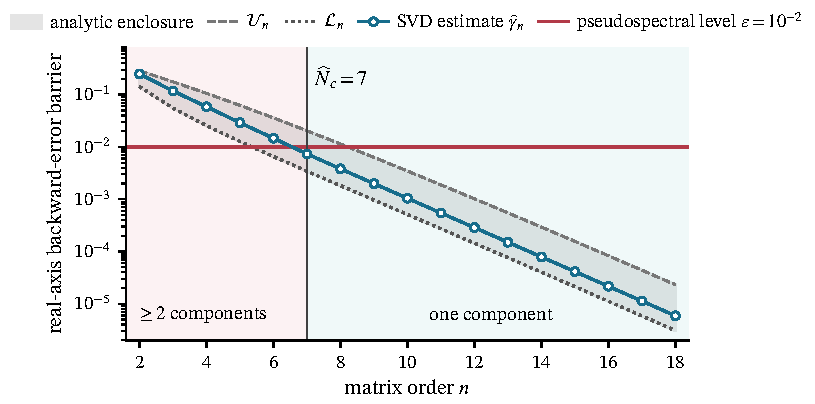
\includegraphics[width=.84\textwidth]{fig2_gap_barrier_bounds}
 \caption{Real-axis backward-error barriers for \(a=1/4\).
 The gray band, bounded by the dotted lower curve \(\mathcal L_n(a)\) and
 dashed upper curve \(\mathcal U_n(a)\), is the rigorous enclosure of
 \(\gamma_n\) and establishes the order \((n+1)a^{n/2}\).  Blue circles joined by
 a solid line are floating-point estimates; the red horizontal line is the
 fixed pseudospectral level \(\varepsilon=10^{-2}\), and the black vertical line marks
 the numerical crossing \(\widehat N_c=7\).  The theorem gives the bracket
 \(6\leq N_c\leq9\).}
 \label{fig:barriers}
\end{figure}

\section{Discussion}\label{sec:discussion}

The boundary regimes are singular limits of the nonnormal interior: the
threshold scale changes from \(c(n+1)a^{n/2}\) for \(0<a<1\) to
\(\pi c/(n+1)\) at \(a=1\) and zero at \(a=0\).  Accordingly, the remainder
\(O_a(1)\) in \eqref{eq:N-asymptotic-main} is pointwise in fixed \(a\) and
loses uniformity near the boundaries.

For every irreducible family, the connected orders form an integer tail with
initial index \(N_T(\alpha,d,\beta;\varepsilon)\); at the reducible boundary,
the tail begins at \(n=2\).

The vertical-contraction theorem separates the transferable topology from
the Toeplitz-specific algebra.  For another matrix family with spectrum on an
affine line, contraction toward that line yields component contractibility
and a one-dimensional connectedness criterion.  Adjacent-order comparison
then becomes a problem for the resulting barrier; in the present family it is
resolved by folded continuants and chord geometry.

We use the Euclidean vector norm and the corresponding full ball of complex
perturbations in the induced operator norm.  Structured variants generally
have different connectedness thresholds; see
\cite{ButtaGuglielmiNoschese2012} for Toeplitz-structured pseudospectra.
Block Toeplitz matrices and periodic \(k\)-Toeplitz families are natural
settings for extending the order comparison.

Restricting the nearest-neighbor Hatano--Nelson hopping law
\cite{HatanoNelson1996,HatanoNelson1997} to an open finite chain and, if
necessary, reversing its orientation gives, up to sign and scale,
\(A_n(a)\), with \(t_L\geq t_R>0\) and \(a=t_R/t_L\).  Its reciprocal
case is the normal boundary, its one-way limit is the Jordan boundary, and
its nonreciprocal interior is the nonnormal regime.  Writing
\(h=\tfrac12\log(t_L/t_R)\), the closed-form tridiagonal Toeplitz
eigenvectors give the right-eigenvector envelope \(e^{-h(j-1)}\)
\cite{NoschesePasquiniReichel2013}; analogous exponential edge localization
of the nontrivial modes is proved for a finite gauge-capacitance chain in
\cite{AmmariEtAl2024}.
The same exponent appears in \(a^{n/2}=e^{-hn}\).  Thus eigenvector
localization and pseudospectral connectedness share the same exponential
scale in the nonreciprocal chain.

\appendix
\renewcommand{\thetheorem}{\Alph{section}.\arabic{theorem}}

\section{Pentadiagonal continuant certificate for vertical monotonicity}
\label[appendix]{app:vertical-certificate}

\begin{proposition}[Vertical determinant certificate]
\label[proposition]{prop:vertical-determinant-certificate}
Fix \(0<a<1\), \(x\in\mathbb R\), \(Y\geq0\), and \(t\in\mathbb R\), and
extend the matrix notation by
\(A_1=[0]\).  For \(k\geq1\), set
\[
 \begin{aligned}
 \mathcal P_k(Y,t)
 &=((x+\ii\sqrt Y)I_k-A_k)^*((x+\ii\sqrt Y)I_k-A_k)-t^2I_k,\\
 F_k(Y,t)&=\det\mathcal P_k(Y,t),
 \end{aligned}
\]
and set \(F_0=1\).  For every \(n\geq1\),
\[
 \mathcal P_n(Y,t)>0
 \quad\Longrightarrow\quad
 \partial_YF_n(Y,t)>0.
\]
\end{proposition}

\begin{proof}
At a fixed value of \(Y\), write
\[
 \delta_{\rm pent}=x^2+Y+1+a^2-t^2,
 \qquad b=-(1+a)x+\ii(1-a)\sqrt Y.
\]
For \(n\geq2\), the matrix \(\mathcal P_n(Y,t)\) has diagonal
\[
 \delta_{\rm pent}-1,\delta_{\rm pent},\ldots,\delta_{\rm pent},
 \delta_{\rm pent}-a^2,
\]
whereas for \(n=1\) its sole entry is
\(\delta_{\rm pent}-1-a^2\).  In all dimensions
its first upper diagonal is \(b\), its first lower diagonal is \(\bar b\),
and its second off-diagonals are \(a\).  Let \(T_k\) be the determinant of
the pure pentadiagonal Toeplitz matrix with diagonal
\(\delta_{\rm pent}\) and these two
off-diagonals.  Set \(T_{-1}=0,T_0=1\), and put
\begin{equation}\label{eq:D-R-def}
 D_k=T_k-T_{k-1},\qquad R_k=T_k-a^2T_{k-1}.
\end{equation}
Since a determinant is affine in each diagonal entry, replacing the
first diagonal entry \(\delta_{\rm pent}\) by
\(\delta_{\rm pent}-1\) subtracts the cofactor \(T_{k-1}\), whereas
replacing the last one by \(\delta_{\rm pent}-a^2\) subtracts
\(a^2T_{k-1}\).  Thus, for \(k<n\), \(D_k\) and \(R_k\) are,
respectively, the leading and trailing principal minors of
\(\mathcal P_n(Y,t)\).

The following continuant calculation isolates all dependence on \(Y\).
With \(T_k=0\) for \(k<0\), a Laplace expansion over the last two rows,
grouped according to the largest displaced index in the contributing
permutation, gives for every \(k\geq1\)
\begin{equation}\label{eq:T-recurrence}
\begin{aligned}
T_k={}&\delta_{\rm pent}T_{k-1}-(|b|^2-a^2)T_{k-2}
-\bigl(2a^2\delta_{\rm pent}-a(b^2+\bar b^2)\bigr)T_{k-3}\\
&-a^2(|b|^2-a^2)T_{k-4}+a^4\delta_{\rm pent}T_{k-5}-a^6T_{k-6}
-a^2\boldsymbol 1_{\{k=2\}}.
\end{aligned}
\end{equation}
For example, \(T_1=\delta_{\rm pent}\) and
\(T_2=\delta_{\rm pent}^2-|b|^2\); these also verify the
only inhomogeneous coefficient in \eqref{eq:T-recurrence}.  Multiplying
the recurrence by \(z^k\) and summing gives
\begin{equation}\label{eq:T-generating}
 \sum_{k\geq0}T_kz^k=\frac{1-a^2z^2}{Q(z,Y)},
\end{equation}
where
\[
\begin{aligned}
 Q(z,Y)={}&1-\delta_{\rm pent}z+(|b|^2-a^2)z^2
 +\bigl(2a^2\delta_{\rm pent}-a(b^2+\bar b^2)\bigr)z^3\\
 &+a^2(|b|^2-a^2)z^4-a^4\delta_{\rm pent}z^5+a^6z^6.
\end{aligned}
\]
Substituting \eqref{eq:T-generating} into \eqref{eq:D-R-def}, with
\(\mathcal D(z,Y)=\sum_{k\geq0}D_kz^k\), gives the first identity in
\begin{equation}\label{eq:D-F-generating}
 \mathcal D(z,Y)=\frac{(1-z)(1-a^2z^2)}{Q(z,Y)},\qquad
 \sum_{k\geq0}F_k(Y,t)z^k=(1-a^2z)\mathcal D(z,Y).
\end{equation}
For the second identity in \eqref{eq:D-F-generating}, first change the initial diagonal, producing
\(D_k\), and then change the final diagonal; its cofactor is
\(D_{k-1}\).  Thus \(F_k=D_k-a^2D_{k-1}\), which proves the asserted
generating function.  Direct substitution of \(\delta_{\rm pent}\) and \(b\) gives
\[
 \partial_YQ=-z(1-z)(1+az)^2(1-a^2z).
\]
Differentiating \eqref{eq:D-F-generating} therefore yields
\begin{equation}\label{eq:F-prime-generating}
 \sum_{k\geq0}\partial_YF_k(Y,t)z^k
 =\varphi_a(z)\mathcal D(z,Y)^2,
 \qquad
 \varphi_a(z)=\frac{z(1+az)(1-a^2z)^2}{1-az}.
\end{equation}

Suppose that \(\mathcal P_n(Y,t)>0\).  Then
\begin{equation}\label{eq:D-R-positive}
 D_k>0,\qquad R_k>0\qquad(0\leq k<n).
\end{equation}
Under the positivity in \eqref{eq:D-R-positive}, put
\(u_k=\sum_{j=0}^kD_jD_{k-j}\), with \(u_k=0\) for \(k<0\).
To extract coefficients from \eqref{eq:F-prime-generating}, note that the
coefficients of \(\varphi_a\), beginning with the coefficient of
\(z\), are
\[
 1,\quad 2a(1-a),\quad a^2(a^2-4a+2),\quad
 2a^{k-1}(1-a)^2\quad(k\geq4).
\]
Thus
\begin{equation}\label{eq:F-prime-convolution}
\begin{aligned}
 \partial_YF_n={}&u_{n-1}+2a(1-a)u_{n-2}
 +a^2(a^2-4a+2)u_{n-3}\\
 &+2(1-a)^2\sum_{k=4}^na^{k-1}u_{n-k}.
\end{aligned}
\end{equation}

The third coefficient is the sole term that may be negative; the following
cofactor inequality controls its contribution.  Let \(j,k\geq1\),
\(j+k=n-1\).  Deleting index \(k+1\) from \(\mathcal P_n\) leaves blocks of
sizes \(k\) and \(j\), with the second off-diagonal \(a\) as their sole
coupling.  In block form, the deleted principal submatrix is
\[
 \begin{bmatrix}
  L_k&a \mathbf e_k\mathbf e_1^T\\
  a \mathbf e_1\mathbf e_k^T&R_j^{\rm mat}
 \end{bmatrix},
 \qquad \det L_k=D_k,\quad \det R_j^{\rm mat}=R_j.
\]
Expanding once in each of the two coupling entries shows that its
determinant is
\begin{equation}\label{eq:deleted-cofactor}
 D_kR_j-a^2D_{k-1}R_{j-1}>0.
\end{equation}
Deleting index \(j+1\) instead gives the same inequality with \(j,k\)
interchanged.  Define
\[
 \vartheta_k=\frac{D_k}{D_{k-1}},\qquad
 \varpi_k=\frac{R_k}{R_{k-1}}.
\]
Since \(T_k=\sum_{\ell=0}^kD_\ell\), \eqref{eq:D-R-def} gives
\begin{equation}\label{eq:R-D-relation}
 R_k=D_k+(1-a^2)\sum_{\ell=0}^{k-1}D_\ell,\qquad
 R_k-R_{k-1}=D_k-a^2D_{k-1}.
\end{equation}
The second identity in \eqref{eq:R-D-relation} shows that
\(\vartheta_k\leq a^2\) implies \(\varpi_k\leq1\).  On dividing
\eqref{eq:deleted-cofactor} and its companion by positive factors, we
obtain
\begin{equation}\label{eq:ratio-cross}
 \vartheta_k\varpi_j>a^2,\qquad \vartheta_j\varpi_k>a^2.
\end{equation}
If both \(\vartheta_j\) and \(\vartheta_k\) were at most \(a^2\), then
both \(\varpi_j\) and \(\varpi_k\) would be at most \(1\),
contradicting \eqref{eq:ratio-cross}.  Hence, after interchanging
\(j,k\) if necessary, \(\vartheta_j>a^2\).  Moreover,
\[
 \vartheta_jR_{j-1}-a^2R_j
 =(\vartheta_j-a^2)(R_{j-1}-a^2D_{j-1}),
\]
and the second factor equals
\((1-a^2)\sum_{\ell=0}^{j-1}D_\ell>0\).  Therefore
\[
 \vartheta_j>a^2\quad\Longrightarrow\quad
 \varpi_j<\vartheta_j/a^2.
\]
The first inequality in \eqref{eq:ratio-cross} now gives
\(a^2<\vartheta_k\varpi_j<\vartheta_j\vartheta_k/a^2\), and therefore
\begin{equation}\label{eq:D-ratio-product}
 \vartheta_j\vartheta_k>a^4.
\end{equation}
Consequently, for \(n\geq3\),
applying \eqref{eq:D-ratio-product} to \(j=p+1\), \(k=n-2-p\) gives
\[
 D_{p+1}D_{n-2-p}>a^4D_pD_{n-3-p},
 \qquad0\leq p\leq n-3.
\]
Summing and then adding the two positive endpoint terms gives
\begin{equation}\label{eq:u-absorption}
 u_{n-1}=2D_{n-1}+\sum_{j=1}^{n-2}D_jD_{n-1-j}>a^4u_{n-3}.
\end{equation}

If the third coefficient in \eqref{eq:F-prime-convolution} is negative,
write it as \(-\mathcal B_{\rm neg}\), where
\(\mathcal B_{\rm neg}=a^2(4a-2-a^2)\).  Since
\[
 a^4-\mathcal B_{\rm neg}=2a^2(1-a)^2>0,
\]
equations \eqref{eq:F-prime-convolution} and \eqref{eq:u-absorption}
prove \eqref{eq:det-derivative-positive}.  If that coefficient is
nonnegative, the implication follows directly.  For \(n=1\), one has
\(\partial_YF_1=1\); for \(n=2\), one has
\(\partial_YF_2=2D_1+2a(1-a)>0\).  Thus
\eqref{eq:det-derivative-positive} holds in every dimension, which proves
the proposition.
\end{proof}

\section{Folded-continuant transfer and boundary residuals}
\label[appendix]{app:folded-transfer}

This appendix derives the transfer and generating identities underlying
\eqref{eq:fold-even}--\eqref{eq:fold-odd} and tracks the boundary signs and
parity conventions in the signed-pencil argument.
Pair the coordinates in the order
\((1,n),(2,n-1),\ldots\).  In this order the symmetric matrix
\((xI_n-A_n)J_n-sI_n\) is block tridiagonal.  Its interior diagonal and
off-diagonal blocks are
\[
 D_{\rm int}=\begin{bmatrix}-s&x\\x&-s\end{bmatrix},
 \qquad
 E_{\rm off}=\begin{bmatrix}0&-1\\-a&0\end{bmatrix},
\]
with lower block \(E_{\rm off}^T\).  For even order the terminal block is
\[
 D_{\rm term}^{\rm e}=\begin{bmatrix}-1-s&x\\x&-a-s\end{bmatrix};
\]
for odd order the terminal block is the scalar \(x-s\), coupled to the
preceding block by the column \((-1,-a)^T\).  Since
\[
 (xI_n-A_n-sJ_n)=\bigl((xI_n-A_n)J_n-sI_n\bigr)J_n,
\]
the determinant of this block matrix, multiplied by \(\det J_n\), is
\(q_n(x,s)\).  Set \(\mathcal Q_m^{\rm e}=q_{2m}(x,s)\) and
\(\mathcal Q_m^{\rm o}=q_{2m+1}(x,s)\).  The following five-minor transfer
completes the continuant verification.
For \(\tau\in\{\mathrm e,\mathrm o\}\), let \(K_m^\tau\) denote the
corresponding matrix
\[
 (xI_n-A_n-sJ_n)J_n=(xI_n-A_n)J_n-sI_n,
 \qquad n=2m\ \text{or}\ 2m+1,
\]
after simultaneously permuting its rows and columns into the paired
order.  Thus \(K_m^{\mathrm e}\) has order \(2m\),
\(K_m^{\mathrm o}\) has order \(2m+1\), and
\[
 K_1^{\mathrm e}=
 \begin{bmatrix}-1-s&x\\x&-a-s\end{bmatrix},
 \qquad
 K_1^{\mathrm o}=
 \begin{bmatrix}
 -s&x&-1\\
 x&-s&-a\\
 -1&-a&x-s
 \end{bmatrix}.
\]
For \(m\geq1\), increasing \(m\) by one adds one interior block at the
exposed end:
\begin{equation}\label{eq:fold-block-extension}
 K_{m+1}^\tau=
 \begin{bmatrix}
  D_{\rm int}&\mathcal E_m^\tau\\
  (\mathcal E_m^\tau)^T&K_m^\tau
 \end{bmatrix},
 \qquad
 \mathcal E_m^\tau=
 \begin{bmatrix}E_{\rm off}&0\end{bmatrix},
\end{equation}
where the zero block has the width required by \(K_m^\tau\).

For a matrix whose first two coordinates are exposed, write
\(K(\widehat I\mid\widehat J)\) for the matrix obtained by deleting
rows \(I\) and columns \(J\).  Suppressing the parity superscript, set
\[
\begin{aligned}
 \mathfrak d_m&=\det K_m,&
 \mathfrak p_m&=\det K_m(\widehat1\mid\widehat1),&
 \mathfrak q_m&=\det K_m(\widehat2\mid\widehat2),\\
 \mathfrak c_m&=\det K_m(\widehat1\mid\widehat2),&
 \mathfrak r_m&=\det K_m(\widehat{1,2}\mid\widehat{1,2}).
\end{aligned}
\]
The off-principal minor obtained by deleting row \(2\) and column \(1\)
has the same value \(\mathfrak c_m\), because \(K_m\) is symmetric.

The one-step transfer follows from a Schur complement.  On the dense set
where both \(K_m\) and the tail obtained by deleting its first two
coordinates are invertible, let
\[
 F=\begin{bmatrix}u&w\\w&v\end{bmatrix}
\]
be its Schur complement in \(K_m\), and let \(\delta\) be the
determinant of that tail.  Then
\[
 (\mathfrak d_m,\mathfrak p_m,\mathfrak q_m,\mathfrak c_m,\mathfrak r_m)
 =\delta(uv-w^2,v,u,w,1).
\]
Since
\[
 E_{\rm off}\operatorname{adj}(F)E_{\rm off}^T
 =
 \begin{bmatrix}u&-aw\\-aw&a^2v\end{bmatrix},
\]
taking the Schur complement of \(K_m\) in
\eqref{eq:fold-block-extension} gives
\begin{equation}\label{eq:five-minor-update}
\begin{aligned}
 \mathfrak d_{m+1}
 &= (s^2-x^2)\mathfrak d_m
    +s(a^2\mathfrak p_m+\mathfrak q_m)
    -2ax\mathfrak c_m+a^2\mathfrak r_m,\\
 \mathfrak p_{m+1}&=-s\mathfrak d_m-a^2\mathfrak p_m,\\
 \mathfrak q_{m+1}&=-s\mathfrak d_m-\mathfrak q_m,\\
 \mathfrak c_{m+1}&=x\mathfrak d_m+a\mathfrak c_m,\\
 \mathfrak r_{m+1}&=\mathfrak d_m.
\end{aligned}
\end{equation}
Both sides are polynomial in \(x\) and \(s\).  For each fixed \(0<a<1\),
the identities hold on a dense nonsingular set, so the polynomial identity
theorem extends them to all \(x,s\), including singular matrix cases.

The five quantities in \eqref{eq:five-minor-update} satisfy one linear
invariant.  Define
\[
 \ell_m=(1-a)\mathfrak d_m-as\,\mathfrak p_m+s\,\mathfrak q_m
       +(1-a)x\mathfrak c_m-a(1-a)\mathfrak r_m.
\]
Direct substitution into \eqref{eq:five-minor-update} gives
\[
 \ell_{m+1}=-a\ell_m.
\]
For the two terminal blocks, direct evaluation gives
\[
\begin{aligned}
&(\mathfrak d_1,\mathfrak p_1,\mathfrak q_1,\mathfrak c_1,\mathfrak r_1)_{\mathrm e}\\
&\qquad=\bigl((1+s)(a+s)-x^2,-a-s,-1-s,x,1\bigr),\\
&(\mathfrak d_1,\mathfrak p_1,\mathfrak q_1,\mathfrak c_1,\mathfrak r_1)_{\mathrm o}\\
&\qquad=\bigl(x(1+a^2)+2as-C_0(x-s),\\
&\hspace{26mm}s^2-sx-a^2,\ s^2-sx-1,\ x^2-sx-a,\ x-s\bigr).
\end{aligned}
\]
Thus \(\ell_1=0\) in both parity classes, and consequently
\begin{equation}\label{eq:fold-minor-invariant}
 (1-a)\mathfrak d_m-as\,\mathfrak p_m+s\,\mathfrak q_m
 +(1-a)x\mathfrak c_m-a(1-a)\mathfrak r_m=0
 \qquad(m\geq1).
\end{equation}

Because
\[
 \det J_{2m}=\det J_{2m+1}=(-1)^m,
\]
the first coordinate of the following signed state is the required
determinant:
\[
 \boldsymbol\eta_m^\tau
 =
 (-1)^m
 \begin{bmatrix}
 \mathfrak d_m^\tau&\mathfrak p_m^\tau&
 \mathfrak q_m^\tau&\mathfrak c_m^\tau
 \end{bmatrix}^{T},
 \qquad
 (\boldsymbol\eta_m^{\mathrm e})_1=\mathcal Q_m^{\mathrm e},
 \quad
 (\boldsymbol\eta_m^{\mathrm o})_1=\mathcal Q_m^{\mathrm o}.
\]
Eliminating \(\mathfrak r_m\) with \eqref{eq:fold-minor-invariant} reduces
\eqref{eq:five-minor-update} to the four-dimensional transfer
\begin{equation}\label{eq:fold-four-transfer}
 \boldsymbol\eta_{m+1}^\tau
 =\mathsf T_{\rm fold}\boldsymbol\eta_m^\tau,
 \qquad
 \mathsf T_{\rm fold}=
 \begin{bmatrix}
 x^2-s^2-a&\dfrac{a^3s}{1-a}&-\dfrac{s}{1-a}&ax\\[2mm]
 s&a^2&0&0\\
 s&0&1&0\\
 -x&0&0&-a
 \end{bmatrix}.
\end{equation}
Set
\begin{equation}\label{eq:fold-transfer-initial}
 \boldsymbol\eta_0^{\mathrm e}
 =\begin{bmatrix}1&a^{-1}&1&0\end{bmatrix}^{T},
 \qquad
 \boldsymbol\eta_0^{\mathrm o}
 =\begin{bmatrix}x-s&1&1&-1\end{bmatrix}^{T}.
\end{equation}
These values incorporate the terminal conditions at \(m=0\).
Direct multiplication in \eqref{eq:fold-four-transfer} reproduces the
signed terminal minors above.  Hence
\(\boldsymbol\eta_m^\tau
=\mathsf T_{\rm fold}^{\,m}\boldsymbol\eta_0^\tau\) for every
\(m\geq0\).

A direct determinant calculation gives
\begin{equation}\label{eq:fold-transfer-characteristic}
\begin{aligned}
 \det(\lambda I_4-\mathsf T_{\rm fold})
 &=
 \lambda^4-C_0\lambda^3+\mathfrak b\lambda^2
 -a^2C_0\lambda+a^4,\\
 \mathfrak b
 &=(1+a^2)x^2+2as^2+2a^2-2a-2a^3.
\end{aligned}
\end{equation}
Apply Cayley--Hamilton with the characteristic polynomial
\eqref{eq:fold-transfer-characteristic} to \(\mathsf T_{\rm fold}\), multiply by
\(\mathsf T_{\rm fold}^{\,m-4}\boldsymbol\eta_0^\tau\), and extract the
first coordinate.  For both \(Z_m=\mathcal Q_m^{\mathrm e}\) and
\(Z_m=\mathcal Q_m^{\mathrm o}\), this yields
\begin{equation}\label{eq:fold-recurrence}
 Z_m-C_0Z_{m-1}+\mathfrak bZ_{m-2}
 -a^2C_0Z_{m-3}+a^4Z_{m-4}=0,
 \qquad m\geq4.
\end{equation}

Applying \(\mathsf T_{\rm fold}\) three times to
\eqref{eq:fold-transfer-initial} gives the initial residuals for the
recurrence \eqref{eq:fold-recurrence}:
\[
 \mathsf{Res}_0=Z_0,\quad
 \mathsf{Res}_1=Z_1-C_0Z_0,\quad
 \mathsf{Res}_2=Z_2-C_0Z_1+\mathfrak bZ_0,
\]
\[
 \mathsf{Res}_3
 =Z_3-C_0Z_2+\mathfrak bZ_1-a^2C_0Z_0,
\]
namely
\[
\begin{array}{ccccc}
 \toprule
 &\mathsf{Res}_0&\mathsf{Res}_1&\mathsf{Res}_2&\mathsf{Res}_3\\ \midrule
 Z_m=\mathcal Q_m^{\rm e}
 &1&a(1-2\zeta_s)&a^2(1-2\zeta_s)&a^3\\
 Z_m=\mathcal Q_m^{\rm o}
 &x-s&-[x(1+a^2)+2as]&a^2(x-s)&0\\
 \bottomrule
\end{array}.
\]
Thus, as a formal-power-series identity,
\[
 \Pi(z)\sum_{m\geq0}Z_mz^m
 =\mathsf{Res}_0+\mathsf{Res}_1z+\mathsf{Res}_2z^2+\mathsf{Res}_3z^3.
\]
For the even sequence the polynomial on the right factors as
\((1+az)(1-2a\zeta_sz+a^2z^2)\); for the odd sequence it is
\((x-s)-[x(1+a^2)+2as]z+a^2(x-s)z^2\).  These factorizations identify the
boundary-residual polynomials.  Since \(\Pi(0)=1\), division by \(\Pi\) in
\(\mathbb R[[z]]\) gives the formal-power-series identities
\begin{equation}\label{eq:fold-generating-even}
 \sum_{m\geq0}\mathcal Q_m^{\rm e}z^m
 =(1+az)(1-2a\zeta_sz+a^2z^2)\Pi(z)^{-1},
\end{equation}
and
\begin{equation}\label{eq:fold-generating-odd}
 \sum_{m\geq0}\mathcal Q_m^{\rm o}z^m
 =\bigl((x-s)-[x(1+a^2)+2as]z+a^2(x-s)z^2\bigr)
  \Pi(z)^{-1}.
\end{equation}

\section{Divided differences for the folded Chebyshev formulas}
\label[appendix]{app:half-chord}

The preceding transfer calculation gives two rational
generating functions.  Coefficient extraction converts them to the
divided-difference formulas used in the half-angle chord parametrization.
Fix \(0<a<1\) and set \(U_{-1}=0\).  The Chebyshev generating function gives
\[
 \sum_{m\geq0}(u-\zeta_s)(U_m(u)+U_{m-1}(u))\omega_{\rm gf}^m
 =\frac{(u-\zeta_s)(1+\omega_{\rm gf})}
 {1-2u\omega_{\rm gf}+\omega_{\rm gf}^2},
\]
and, with \(\mathsf B_s^{\rm fold}=[x(1+a^2)+2as]/(2a)\),
\[
 \sum_{m\geq0}((x-s)u-\mathsf B_s^{\rm fold})U_m(u)\omega_{\rm gf}^m
 =\frac{(x-s)u-\mathsf B_s^{\rm fold}}
 {1-2u\omega_{\rm gf}+\omega_{\rm gf}^2}.
\]
Let \(u,v\in\mathbb R\) satisfy the two symmetric relations in
\eqref{eq:fold-characteristic}.  Taking the corresponding divided
difference of the Chebyshev generating identities and putting
\(\omega_{\rm gf}=az\) recovers
\eqref{eq:fold-generating-even} and \eqref{eq:fold-generating-odd}.
Coefficient comparison gives \eqref{eq:fold-even}--\eqref{eq:fold-odd},
including the derivative value when \(u=v\).  The underlying polynomial
identities remain valid when \(\Delta_{\rm fold}<0\), without choosing a
square-root branch.

\section{Exhaustion of the endpoint-side chord sheet}
\label[appendix]{app:chord-exhaustion}

This appendix proves the chord-sheet exhaustion lemma used in the main
comparison.

\begin{proof}[Proof of \Cref{lem:chord-sheet-exhaustion}]
Continue the ordered middle root \(s_*(x)\) through the open gap.  Write
\(\Delta_*(x)=\Delta_{\rm fold}(x,s_*(x))\) for its folded discriminant,
let \(y(x)\leq z(x)\) be the reconstructed nonnegative half variables on
the real sheet issuing from the endpoint germ, and set
\(\theta_{\rm ch}(x)=\arccos y(x)\).  Let \(\mathcal C\) be the set of gap points for
which
\[
 \Delta_*(x)>0,\qquad
 \frac{j\pi}{K}<\theta_{\rm ch}(x)<\frac{(j+1)\pi}{K},\qquad
 u_K^{\max}<z(x)<\mathfrak c_h.
\]
On \(\mathcal C\), the reversible folded determinant identities give
\(\mathcal W_K(y(x))=\mathcal W_K(z(x))\); uniqueness on the endpoint-side
outer lobe then gives
\[
 z(x)=z_K(\mathcal W_K(y(x))).
\]
Thus \(\mathcal C\) is precisely the selected endpoint-side chord sheet.
At the upper gap endpoint, \(z=\mathfrak c_h\) and
\(\theta_{\rm ch}=j\pi/K\).  There
\(z=\mathfrak c_h>1\geq y\), so \(\Delta_*>0\) persists immediately
inside the gap.  Moreover,
\cref{lem:middle-branch} gives \(\operatorname{sgn}s_*=(-1)^j\); the signed
chord equation therefore places
\(\theta_{\rm ch}\) in
\((j\pi/K,(j+1)\pi/K)\).  Since \(|s_*|>0\), the channel identity gives
\(z<\mathfrak c_h\), while continuity keeps \(z>u_K^{\max}\).  Hence
\(\mathcal C\) is nonempty.  The ordered eigenvalues of the continuous real symmetric pencil
\(B_{K-1}(x)\) are continuous in \(x\), including at an eigenvalue crossing,
so the continuation passes through a multiple least singular value.  The
folded pair \(u=2z^2-1\), \(v=2y^2-1\) and its reconstructed half variables
are continuous, while the sheet inequalities are strict.  Thus
\(\mathcal C\) is relatively open in the gap.

It is also relatively closed.  At a relative closure point the chord
identity and all sheet inequalities persist weakly.  The possible closure
cases are as follows.  (1) If \(\Delta_*(x)=0\), then the reconstructed half
variables coincide, which is impossible because
\[
 z\geq u_K^{\max}>\cos\frac{\pi}{K}
 \geq\cos\frac{j\pi}{K}\geq y.
\]
(2) At an interior point of a positive gap, including one adjacent to zero,
both half variables retain their signs: \(z>0\), while \(y=0\) would force
\(x=0\), outside the open positive half.  (3) Neither the outer variable can
reach \(\mathfrak c_h\) nor the inner variable a nodal endpoint: in either
case the common level is zero, the endpoint-side solution is
\(z=\mathfrak c_h\), and \eqref{eq:channel-xs} gives \(s=0\), impossible
inside a spectral gap.  (4) The
outer variable remains in its endpoint-side component, since its first exit
point would be \(u_K^{\max}\), contradicting
\eqref{eq:outer-level-dominates}.  Passage through \(z=1\) changes only the
coordinate representation.  Hence every relative closure point remains in
\(\mathcal C\).  Since the open gap is an interval, \(\mathcal C\) is the
entire gap.  This proves the first exhaustion direction: every actual gap
point lies on the selected endpoint-side chord sheet.

For the converse direction, the reconstructed angle \(\theta_{\rm ch}\) extends
continuously to the closed spectral gap.  The exact folded variables at the
two endpoints give
\[
 \theta_{\rm ch}(\lambda_{K-1,j+1})=\frac{(j+1)\pi}{K},\qquad
 \theta_{\rm ch}(\lambda_{K-1,j})=\frac{j\pi}{K}.
\]
For every \(\theta_0\in(j\pi/K,(j+1)\pi/K)\), the intermediate value
theorem therefore supplies an interior gap point \(x\) with
\(\theta_{\rm ch}(x)=\theta_0\).  The preceding classification and uniqueness of
the endpoint-side outer solution then give
\[
 y(x)=\cos\theta_0,\qquad
 z(x)=z_K(\mathcal W_K(\cos\theta_0)),
\]
so the corresponding abscissa and signed root are exactly those of the
prescribed \(j\)-chord.  Thus every chord parameter produces an actual point
of the ordered middle branch.  By \cref{lem:middle-branch}, its positive
magnitude is \(s_{\min}(xI_{K-1}-A_{K-1})\).

When \(K\) is odd, the same argument applies to the positive half of
the single central gap, continuing from the positive spectral endpoint
to \(x=0\).  Because \(z>0\), the identity
\(x=(2r/\mathfrak c_h)\cos\theta\,z\) forces \(\theta=\pi/2\) at
\(x=0\).  Thus every parameter on that half occurs, and reflection covers
the negative half.
\end{proof}

\section{Scalar estimate for the lower central-gap comparison}
\label[appendix]{app:central-scalar}

This appendix proves \eqref{eq:central-target} separately in the regimes
\(\rho>1\), \(\rho=1\), and \(\rho<1\).

Put \(b=u_+/u_-=1/a\), and define
\[
 Q_b=b^2-2b\rho+1,\qquad S_b=b^2+2b\omega_L+1.
\]
The Chebyshev identity gives \(u_-^2Q_b=1\), and
\begin{equation}\label{eq:central-D-QS}
 \mathfrak D_L=S_b/Q_b,\qquad
 \Delta_\xi:=\rho-\xi=\Delta_\omega Q_b/S_b.
\end{equation}
Indeed, since \(u_+=bu_-\) and \(u_-^2=Q_b^{-1}\),
\[
 \mathfrak D_L=1+2(\rho+\omega_L)u_-u_+
  =1+\frac{2b(\rho+\omega_L)}{Q_b}=\frac{S_b}{Q_b},
\]
which proves the first identity in \eqref{eq:central-D-QS}; the second
follows from
\eqref{eq:central-D-xi}.
The ratio \(U_L/U_{L-1}\) is strictly increasing above the largest zero
of \(U_{L-1}\), and equals \(1\) at
\(\rho_{\rm ref}=\cos\frac{\pi}{2L+1}\).  Hence
\(\rho>\rho_{\rm ref}\).  Since
\(S_b-Q_b=2b(\rho+\omega_L)>0\),
\[
 \xi>\rho_{\rm ref}-\Delta_\omega>2\omega_L-1
 >2\omega_L^2-1=\cos\frac{\pi}{L}.
\]
Therefore \(f_L(x)=(1+x)U_{L-1}(x)\) is positive, strictly increasing,
and strictly log-concave on \([\xi,\rho]\).  In particular,
\(\mathfrak d_\rho=(\log f_L)'(\rho)>0\), and
\[
 \mathfrak d_\rho=
 \begin{cases}
  \dfrac{L(b-\rho)-1}{\rho^2-1},&\rho\neq1,\\[6pt]
  \dfrac{2L^2+1}{6},&\rho=1
 \end{cases}.
\]
The endpoint value follows directly from \(U_{L-1}(1)=L\) and
\(U_{L-1}'(1)=L(L^2-1)/3\).  Moreover,
\[
 \log f_L(\rho)-\log f_L(\xi)>\Delta_\xi\mathfrak d_\rho,
 \qquad
 f_L(\xi)^2<f_L(\rho)^2e^{-2\Delta_\xi\mathfrak d_\rho}
 <\frac{f_L(\rho)^2}{1+2\Delta_\xi\mathfrak d_\rho}.
\]
Here the first strict inequality is the integral form of strict
log-concavity.  Since
\(f_L(\rho)^2=(1+\rho)^2/Q_b\) and
\(\Delta_\xi=\Delta_\omega Q_b/S_b\), substitution into
\eqref{eq:central-target} reduces it to
\begin{equation}\label{eq:N-positive-target}
 \mathcal N=(\rho+\omega_L)
 (S_b+2\Delta_\omega Q_b\mathfrak d_\rho)
 -(1+\omega_L)(1+\rho)^2>0.
\end{equation}
All three cases use
\begin{equation}\label{eq:Delta-omega-basic-bound}
 \Delta_\omega=1-\cos\frac{\pi}{2L}
 <\frac{\pi^2}{8L^2}<\frac5{4L^2},
 \qquad \Delta_\omega L<1.
\end{equation}

Suppose first that \(\rho>1\).  Put \(u=b-\rho\) and
\(\Delta_+=\rho^2-1\).  Since \(\mathfrak d_\rho>0\), \(u>1/L\).
Keeping \(\rho\) fixed,
direct differentiation gives
\[
 \frac{\partial_b\mathcal N}{2(\rho+\omega_L)}
 =\rho+\omega_L+u-\Delta_\omega L
 +\frac{\Delta_\omega(3Lu^2-2u)}{\Delta_+}.
\]
The right-hand side is strictly increasing for \(u\geq1/L\) and is positive
at \(u=1/L\) by \eqref{eq:Delta-omega-basic-bound}.  Hence \(\mathcal N\) exceeds
its value at
\(b=\rho+1/L\).  With
\(s_0=\rho+\omega_L\) and \(\omega_+=1+\omega_L\), that value is
\[
 \Upsilon(s_0)
 =s_0\left[\left(s_0+\frac1L\right)^2+\omega_+\Delta_\omega\right]
 -\omega_+(s_0+\Delta_\omega)^2.
\]
For \(s_0\geq\omega_+\),
\[
 \Upsilon''(s_0)=6s_0+4/L-2\omega_+>0,\qquad
 \Upsilon'(\omega_+)=2\omega_L\omega_++4\omega_+/L+1/L^2>0,
\]
and
\[
 \Upsilon(\omega_+)
 =\omega_+(-2\Delta_\omega+2\omega_+/L+1/L^2)>0.
\]
Thus \eqref{eq:N-positive-target} holds when \(\rho>1\).  If \(\rho=1\),
then \(b=(L+1)/L\), \(Q_b=L^{-2}\), and direct substitution, using the
endpoint value of \(\mathfrak d_\rho\), gives
\[
 \mathcal N=\Upsilon(1+\omega_L)
 +\frac{2(1+\omega_L)\Delta_\omega}{L^2}
   \frac{2L^2+1}{6}>0.
\]
The first term is positive by the preceding calculation, and every factor
in the correction term is positive.

For \(\rho<1\), set
\[
 \upsilon=1-\rho,\qquad \Delta_b=b-1,\qquad
 u=\Delta_b+\upsilon,\qquad \Delta_-=\upsilon(2-\upsilon).
\]
Because \(b>1\), we have \(0<\upsilon<u\).  Moreover,
\(\rho^2-1<0\), so the positivity of \(\mathfrak d_\rho\) in its quotient
formula forces \(L(b-\rho)-1<0\).  Since \(u=b-\rho\),
\begin{equation}\label{eq:u-small-range}
 0<\upsilon<u<1/L.
\end{equation}
With \(\rho\) fixed, write \(\mathcal N_\rho^{<}(\mathord\cdot)\) for
\(\mathcal N\) viewed as a function of \(\Delta_b=b-1\).
A direct expansion of \eqref{eq:N-positive-target} gives
\[
 \mathcal N_\rho^{<}(\Delta_b)-\mathcal N_\rho^{<}(0)
 =\frac{\Delta_b(\rho+\omega_L)}{\Delta_-}\mathfrak q(u),
\]
where
\[
 \mathfrak q(u)=\Delta_-[2(2-\Delta_\omega)+u-\upsilon]
 +2\Delta_\omega
 [u+\upsilon-L(u^2+u\upsilon+\upsilon^2)-L\Delta_-].
\]
The function \(\mathfrak q\) is a concave quadratic.  Moreover,
\[
 \mathcal N_\rho^{<}(0)=\frac{\upsilon}{2-\upsilon}
 \bigl[(2-\Delta_\omega)(2-\upsilon)^2
 -2\Delta_\omega^2
 -4\Delta_\omega L(2-\upsilon-\Delta_\omega)\bigr].
\]
The following elementary bounds hold; the second follows from
\(\rho>\rho_{\rm ref}\) and
\(1-\rho_{\rm ref}<\pi^2/[2(2L+1)^2]<5/(2L+1)^2\):
\begin{equation}\label{eq:Delta-upsilon-bounds}
 \Delta_\omega<\frac5{4L^2},\qquad
 \upsilon<\frac5{(2L+1)^2}\leq\frac15.
\end{equation}
When \(L=2\), the non-strict bound equals \(1/5\), while the preceding strict
estimate still gives \(\upsilon<1/5\).  These bounds
in \eqref{eq:Delta-upsilon-bounds} show that the bracketed expression is
positive, since it equals
\[
 (2-\upsilon)
 \bigl[(2-\Delta_\omega)(2-\upsilon)-4\Delta_\omega L\bigr]
 +2\Delta_\omega^2(2L-1)
\]
and, using \(L\geq2\),
\[
 (2-\Delta_\omega)(2-\upsilon)
 >\frac{27}{16}\frac95=\frac{243}{80}
 >\frac52\geq4\Delta_\omega L.
\]
At the endpoints of
\eqref{eq:u-small-range},
\[
 \mathfrak q(\upsilon)=\upsilon
 \bigl[(2-\upsilon)(4-2\Delta_\omega)
 +4\Delta_\omega-4\Delta_\omega L(1+\upsilon)\bigr]>0,
\]
\[
 \mathfrak q(1/L)=\upsilon
 \bigl[(2-\upsilon)(4-2\Delta_\omega+1/L-\upsilon)
 -4\Delta_\omega L\bigr]>0.
\]
At the two endpoints, the positive leading terms exceed
\[
 \frac95\left(4-\frac58\right)=\frac{243}{40},
 \qquad
 \frac95\left(4-\frac58-\frac15\right)=\frac{1143}{200},
\]
while the negative terms have magnitudes less than
\((5/L)(6/5)\leq3\) and \(5/L\leq5/2\), respectively.  Concavity therefore
gives \(\mathfrak q(u)>0\), proving \eqref{eq:N-positive-target}, and hence
\eqref{eq:central-target}, in all three cases.


\section{Signed-root certification in the lower central gap}
\label[appendix]{app:central-certification}

This appendix verifies the folded substitution and
second-singular-value separation used in the main proof of
\(\mathfrak h_m^{\mathrm o}>\mathfrak h_{m+1}^{\mathrm e}\).

At \(x=x_*\) and \(s=\pm\tau_*\), where
\(\tau_*=\mathfrak h_L^{\mathrm e}\), the real pair
\(u=\xi\), \(v=-\omega_L\) satisfies the two symmetric relations in
\eqref{eq:fold-characteristic}.  Indeed, its sum and product are
\(\xi-\omega_L\) and \(-\omega_L\xi\), and the required identities
follow from
\[
 \mathfrak D_L=\frac{\zeta+\omega_L}{\zeta-\rho},\qquad
 \xi=\frac{\rho(\zeta+1)+\zeta(\omega_L-1)}{\zeta+\omega_L}.
\]
Positivity of \(\xi+\omega_L\) selects the distinct-variable branch of the
divided difference in \eqref{eq:fold-odd}.
Write the folded numerator as
\[
 \mathfrak n_s(t)=-[x(\zeta-t)+s(1+t)]U_{L-1}(t).
\]
Put
\[
 \mathsf{X}_\xi=x_*(\zeta-\xi),\quad
 \mathsf{Y}_\xi=\tau_*(1+\xi),\quad
 \mathsf{X}_\omega=x_*(\zeta+\omega_L),\quad
 \mathsf{Y}_\omega=\tau_*\Delta_\omega,
\]
and set \(U_\xi=U_{L-1}(\xi)\),
\(U_{-\omega}=U_{L-1}(-\omega_L)\).  The identities
\[
 \mathfrak D_L=2a(\zeta+\omega_L)u_+^2,\qquad
 \mathfrak D_L(\rho+\omega_L)(\zeta-\xi)
 =(\zeta+\omega_L)(1+\xi)
\]
give
\(\mathsf{Y}_\omega\mathsf{Y}_\xi
=\mathsf{X}_\omega\mathsf{X}_\xi\).  The identity \(u_-^2Q_b=1\) gives
\(Q_b>0\), and \(S_b-Q_b=2b(\rho+\omega_L)>0\), so
\(\mathfrak D_L=S_b/Q_b>1\).  Moreover, \(L\geq2\) gives
\(\omega_L>1/2\), while \(\rho>\rho_{\rm ref}>\omega_L\); hence
\[
 \rho+\omega_L>2\omega_L>1>1-\omega_L>0.
\]
Consequently,
\[
 \frac{\mathsf{X}_\omega^2}{\mathsf{Y}_\omega^2}
 =\frac{\mathfrak D_L(\rho+\omega_L)}{1-\omega_L}>1,
\]
so, with
\(\mathfrak r_*=\mathsf{X}_\xi/\mathsf{Y}_\xi
=\mathsf{Y}_\omega/\mathsf{X}_\omega\in(0,1)\), the common factor
\(a^{L-1}/(\xi+\omega_L)\) in \eqref{eq:fold-odd} is positive, and the two
numerator differences are
\[
\begin{aligned}
 \mathfrak n_{\tau_*}(\xi)-\mathfrak n_{\tau_*}(-\omega_L)
  &=(1+\mathfrak r_*)
    (\mathsf{X}_\omega U_{-\omega}-\mathsf{Y}_\xi U_\xi),\\
 \mathfrak n_{-\tau_*}(\xi)-\mathfrak n_{-\tau_*}(-\omega_L)
  &=(1-\mathfrak r_*)
    (\mathsf{X}_\omega U_{-\omega}+\mathsf{Y}_\xi U_\xi).
\end{aligned}
\]
Their product is positive by \eqref{eq:central-target}, because
\[
 U_{-\omega}^2=\frac1{1-\omega_L^2},\qquad
 \mathsf{X}_\omega^2U_{-\omega}^2
 =\frac{\tau_*^2\mathfrak D_L(\rho+\omega_L)}{1+\omega_L}
 >\mathsf{Y}_\xi^2U_\xi^2.
\]
Thus
\[
 q_{2L-1}(x_*,\tau_*)q_{2L-1}(x_*,-\tau_*)>0.
\]

At \(x=0\), the second-smallest singular value of \(A_{2L-1}\) is
\[
 s_{L,2}^{(0)}=\sqrt{1+a^2-2a\cos\frac{\pi}{L}}.
\]
Indeed, after separating odd and even coordinates, the two rectangular
off-diagonal blocks have Gram matrices equal to the
\((L-1)\)-dimensional tridiagonal Toeplitz matrix with diagonal
\(1+a^2\) and off-diagonal \(a\).  Their singular values therefore have
squares
\[
 1+a^2+2a\cos\frac{k\pi}{L},\qquad 1\leq k\leq L-1,
\]
and each occurs twice, while the remaining singular value is zero.
The required separation is
\[
 x_*+\tau_*<2\sqrt a\sin\frac{\pi}{2L}\leq s_{L,2}^{(0)}.
\]
Indeed, recall \(\rho_{\rm ref}=\cos\frac{\pi}{2L+1}\).  Since
\(\rho>\rho_{\rm ref}\) and \(U_{L-1}\) is strictly increasing above its
largest zero,
\[
 u_-=U_{L-1}(\rho)>U_{L-1}(\rho_{\rm ref})=:u_{-,\rm ref},
 \qquad u_{-,\rm ref}^{-2}=2(1-\rho_{\rm ref}).
\]
The identities \(\tau_*=a/u_-\) and \(\tau_*^2=2a(\zeta-\rho)\) imply
\(\zeta-\rho<a(1-\rho_{\rm ref})<1-\rho_{\rm ref}\).  Also
\[
 \frac{x_*^2}{2a}
 =\Delta_\omega\frac{\rho+\omega_L}{\zeta+\omega_L}
 <\Delta_\omega.
\]
Put
\[
 \theta_L=\frac{\pi}{4L},\qquad
 \Delta_L=\frac{\theta_L}{2L+1}.
\]
Then \(\Delta_\omega=2\sin^2\theta_L\) and
\(1-\rho_{\rm ref}=2\sin^2(\theta_L-\Delta_L)\).  Since all quantities are
positive, the preceding quotient bound for \(x_*^2\) gives
\[
 x_*<2\sqrt a\sin\theta_L.
\]
Likewise,
\[
 \tau_*^2=2a(\zeta-\rho)
 <2a^2(1-\rho_{\rm ref})
 =4a^2\sin^2(\theta_L-\Delta_L),
\]
and hence
\[
 \tau_*<2a\sin(\theta_L-\Delta_L)
 <2\sqrt a\sin(\theta_L-\Delta_L),
\]
where the last inequality uses \(0<a<1\), hence \(a<\sqrt a\).
It suffices to prove
\begin{equation}\label{eq:angle-inequality}
 \sin\theta_L+\sin(\theta_L-\Delta_L)<\sin(2\theta_L).
\end{equation}
The estimates
\[
 2\sin\theta_L-\sin(2\theta_L)
 =2\sin\theta_L(1-\cos\theta_L)<\theta_L^3
\]
and
\[
 \sin\theta_L-\sin(\theta_L-\Delta_L)
 =\int_{\theta_L-\Delta_L}^{\theta_L}\cos u\,du
 >\Delta_L\cos\theta_L
\]
reduce \eqref{eq:angle-inequality} to
\(\Delta_L\cos\theta_L>\theta_L^3\).  Substituting
\(\Delta_L=\theta_L/(2L+1)\) and \(\theta_L=\pi/(4L)\) gives the equivalent
condition \(2\cos\theta_L>\theta_L(\pi+2\theta_L)\).  For
\(0<\theta_L\leq\pi/8\), using \(\pi^2<10\),
\[
 2\cos\theta_L>2-\theta_L^2\geq\frac{59}{32}
 >\frac{25}{16}\geq\theta_L(\pi+2\theta_L).
\]
Consequently \(x_*+\tau_*<2\sqrt a\sin\frac{\pi}{2L}\).  Finally,
\[
 (s_{L,2}^{(0)})^2-4a\sin^2\frac{\pi}{2L}
 =(1-a)^2\geq0,
\]
which proves \eqref{eq:x-c-second-singular}.

Together with the signed product inequality, this proves the signed-root
certification used in \cref{subsec:central-comparison}.

% Project-specific end matter for the LMA manuscript.
% Keep the wording synchronized with the public repository at submission.

\bigskip
\noindent{\bf Funding.}
The author received no specific funding for this work.

\medskip
\noindent{\bf Conflict of interest.}
The author declares no conflict of interest.

\medskip
\noindent{\bf Data and code availability.}
No experimental data or external research datasets were used in this
theoretical study.  The Python code for the numerical illustrations and the
Lean~4 formalization accompanying the mathematical results are available at
\url{https://github.com/jinshanmu/Hatano-Nelson}.

\medskip
\noindent{\bf Acknowledgment of AI-assisted tools.}
During the preparation of this work, the author used OpenAI ChatGPT Work 5.6
Sol for checks of algebraic consistency, presentation, and bibliographic
metadata.  Any resulting revisions were reviewed by the author, who
independently verified all cited references.


\phantomsection
\bibliographystyle{plainurl}
\bibliography{lma_pseudospectral_connectedness}

\end{document}
